% -*- mode: latex; coding: utf-8; fill-column: 72; -*-
% !BIB TS-program = biber
% !BIB program = biber

\documentclass[12pt]{umd-thesis}

\usepackage{graphicx}
\graphicspath{{images/}}

\usepackage{amssymb}
\usepackage{siunitx}
\sisetup{output-exponent-marker=\ensuremath{\mathrm{e}}}
\usepackage{multirow}

\usepackage[american]{babel}

\usepackage{csquotes}

\usepackage[
  backend=biber, style=unified,
  maxcitenames=3, maxbibnames=99]{biblatex}
\addbibresource{references.bib}
% just use a colon as the \postnotedelim
\renewcommand{\postnotedelim}{\addcolon}
\DeclareFieldFormat{postnote}{#1}
% use the Oxford comma
\DeclareDelimFormat{finalnamedelim}{%
  \ifnumgreater{\value{liststop}}{2}{\finalandcomma}{}%
  \addspace\&\space}
% a more sensible way to display the DOI
\DeclareFieldFormat{doi}{%
  \textsc{doi}:
  \ifhyperref
  {\href{http://dx.doi.org/#1}{\nolinkurl{#1}}}
  {\nolinkurl{#1}}}
%quirks of Yu'an:
\newcommand{\citealt}[1]{\cite{#1}}



%%for diagrams/ trees
\usepackage{tikz}
\usepackage{qtree}
\usepackage{tikz-qtree}
\usepackage{pifont} %to crossout movement path 
\usetikzlibrary{arrows,shapes, automata, positioning}
\usetikzlibrary{bayesnet}
\newcommand{\cmark}{\ding{51}}%checkmark
\newcommand{\xmark}{\ding{55}}%xmark

\usepackage{adjustbox}
\usepackage[mode=tex]{standalone}

\usepackage{xcolor}
\definecolor{darkred}{HTML}{B22613}
\definecolor{mygreen}{HTML}{C8DE9C}

\usepackage{gb4e}
\noautomath

\usepackage[colorlinks]{hyperref}
\hypersetup{%
  linkcolor=darkred,
  citecolor=black,
  urlcolor=cyan}

%%%%%%%%%%%%%%%%%%%%%%glossing
\usepackage{textglos}
\usepackage[
  block,
  nohypertypes={main} % option to pass to glossaries package 
]{leipzig}
\newleipzig{dou}{dou}{adverbial quantifier}
\newleipzig{sfp}{sfp}{sentence final particle}
\newleipzig{asp}{asp}{aspect marker}
\newleipzig{qpart}{q}{question particle}
\newleipzig{cl}{cl}{classifier}
%\newleipzig{ind}{ind}{indicative}
\newleipzig{int}{int}{interrogative}
\makeglossaries
%\newacronym{PMC}{PMC}{Principle of Minimal Compliance} %\gls{PMC}
\newacronym{dlearnerabbr}{SID}{Syntactically Informed Distributional Model} %\gls{}
\newacronym{plearnerabbr}{SPID}{Syntactically and Pragmatically Informed Distributional Model}
%%%%%%%%%%%%%%%%%%%%%personalized commands
\usepackage{verbatim}
\usepackage{float}
%gb4e hack
\newcommand{\bex}[1]{\begin{exe}\ex \label{#1}}
\newcommand{\eex}{\end{exe}}
\newcommand{\bxl}{\begin{xlist}\ex}
\newcommand{\exl}{\end{xlist}}

% semantics
\newcommand{\sv}[1]{\left\llbracket#1\right\rrbracket} % [[ ... ]]
\newcommand{\typ}[1]{\left\langle#1\right\rangle} 

%commands for style
\newcommand{\tit}[1]{\textit{#1}}
\newcommand{\tbf}[1]{\textbf{#1}}
\newcommand{\tsc}[1]{\textsc{#1}}
\newcommand{\tun}[1]{\underline{#1}}

%words
\newcommand{\ba}{\textit{ba}}
\newcommand{\ma}{\textit{ma}}
\newcommand{\twh}{\textit{wh}}
\newcommand{\dou}{\textit{dou}}
\newcommand{\twhi}{\textit{wh}-indefinite}
\newcommand{\hypos}{pragmatic bootstrapping hypothesis}
\newcommand{\diis}{declaratives, interrogatives, and imperatives}
\newcommand{\aqrs}{assertions, questions, and requests/commands}
\newcommand{\distlearner}{syntactically informed distributional learner}
\newcommand{\praglearner}{syntactically and pragmatically informed distributional learner}
\newcommand{\dlearnerabbr}{SID}
\newcommand{\plearnerabbr}{SPID}
\newcommand{\subhypo}{pragmatic bootstrapping hypothesis}
\newcommand{\mycode}{\textcolor{red}{url}}



%%%%%%%%%%%%%%%%%%%%%title pages
\title{Learning to identify interrogatives and questions}
\author{Yu'an Yang}
\date{2022}

\cochair{%
  title={Professor}, name={Jeffrey Lidz}, department={Linguistics}}
\chair{%
  title={Professor}, name={Valentine Hacquard}, department={Linguistics}}
\committee{%
  {title={Professor}, name={Yi Ting Huang}, role={Dean's Representative}},
  {title={Professor}, name={Naomi Feldman}, role={}},
  {title={Professor}, name={Alexander Williams}, role={}},
  {title={Dr.}, name={Daniel Goodhue}, role={}}}



\begin{document}
%%%%%%%%%%remember to delete!!!
%%%%%%%%%%%%%%%%%%%%
%\pagecolor{mygreen}
%%%%%%%%%%%%%%%%%%%%%

\frontmatter

\begin{abstract}
  % -*- mode: latex; coding: utf-8; fill-column: 72; -*-

Languages tend to have three major clause types (declaratives, interrogatives, imperatives), dedicated to three main speech acts (assertions, questions, commands). However, the particular forms that these clause types take differ from language to language, and have to be learned. Previous experimental results suggest that by 18 months old, children differentiate these clause types and associate them with their canonical speech act. This dissertation investigates how children learn to identify different clause types and speech acts. 

To learn clause types, children need to identify the right categories of clauses (the "clustering problem") and figure out what speech act they are canonically used for (the "labeling problem"). I investigate the extent to which learners need to rely on pragmatic information (i.e., knowing what speech act a given utterance of sentence is conveying), to solve not just labeling, but the clustering itself. We examine the role of pragmatics computationally by building two Bayesian clustering models. I found that for morpho-syntactic and prosodic information is not enough for identifying the right clause type clustering, pragmatics is necessary. I applied the same model to a morphological impoverished language, Mandarin, and found that the model without pragmatics performs even worse. Speech act information is crucial for finding the right categories. Additionally, a little pragmatics goes a long way. I simulated the learning process with noisy speech act information, and found that noisy speech act information is better than no speech act.

 

But if the speech act information is useful for clause type learning, how do children figure out speech act information? I then explored what kind of non-clause type cues for speech act information are present in the input. Even if children must rely on clause type information to figure out the speech acts, they could have access to additional information that is unrelated to clause typing, but is informative for recognizing speech act type. When speakers perform speech acts, because of the conventional functions of these speech acts on the discourse, the performance might be associated with certain socio-pragmatic features. For example, because of questions' response-elicitation function, we would expect pauses after questions. With prior knowledge about the functions of communication, and expectations about what questions do, children might able to use these socio-pragmatic features to figure out this speech act. 

I explored two cues that could potentially differentiate questions from other speech acts: pauses, and direct eye gaze. I found that parents tend to pause longer after questions, and attend to the child more when asking questions. Therefore it is in principle plausible that there are some socio-pragmatic features that children can use, in addition to their growing knowledge of clause types to infer the speech act category of an utterance. This little bit of information about speech act could then be used to provide enough pragmatic information that the child needs in order to get the clause type clusters identified accurately.
%This dissertation We find (a) that a learner must have access to some pragmatic information in order to find the right clause types but (b) this learner can succeed with very limited access to pragmatic information. 

% Local Variables:
% TeX-engine: xetex
% LaTeX-biblatex-use-Biber: t
% TeX-master: "../main"
% End:

\end{abstract}

\maketitlepage

\makecopyrightpage

\begin{preface}

\end{preface}

\begin{acknowledgments}
  Throughout graduate school, I must have played the scenario of writing this section of the dissertation a thousand times in my head; it always seems so far in the future that it almost seems fictional. I still can’t quite believe that, today is the day that I need to write this part of the dissertation. With sincere apologies to any that I may have forgotten, let me attempt to express my heartfelt thanks to everyone that has taken me to this point.
 
First, my deepest gratitude goes to Valentine Hacquard and Jeff Lidz. Before I even applied to UMD, everyone told me Valentine and Jeff together form a great advising team, and after working with them for five years, I can add my testament to this. Not only did they train me to become a better researcher and a careful thinker, but they were also my cheerleaders. They cheered me on whenever there was any breakthrough, no matter how small it was. I cannot count how many times I was about to give up on an idea, and only pushed through because Valentine and Jeff said “what are you talking about, this is great!” I feel so fortunate to have them as my mentors.
 
Thanks to my committee members, Naomi Feldman, Daniel Goodhue, Alexander Williams, and Yi Ting Huang. I was so nervous when I reached out to Naomi to ask for her help with building a computational model, because I barely understood anything from her class on cognitive modeling. But it turned out that I had nothing to worry about. Naomi was so kind and patient, even when she had to explain to me the extremely basic math for the nth time. Without her, I wouldn’t even dare to ask the ``how” question of learning, and half this dissertation wouldn’t exist. She also connected me with people at the CLIP lab, which saved me so much time. Dan has always been a great mentor, and I had the fortune to both be a mentee, and a co-mentor. I learned so much about mentorship when we worked with a group of undergraduate students together. He always gave the best advice: just challenging enough to make the work better, but not so challenging that you feel defeated. He also always made sure to add some encouragement in his comments, and I’m very grateful for that. Many thanks to Alexander for demonstrating to me how to be a careful thinker. He’d offer the most thoughtful and eloquent comments, often end with a joke that I fail to get (the Chomsky-Wittgenstein-Slab joke still puzzles me). I always wished I had recorded his comments at meetings, so I can write them down verbatim. Being his TA for his Philosophy of Language class was one of the most enlightening experiences for me as a semanticist.
 
I feel so lucky to have spent five years in such an amazing department. This community makes linguistics so much fun, and you know you are in the right place when you look forward to going to work every day. Thank you to Howard Lasnik, for reminding me how breathtakingly beautiful syntax can be, and for giving me the only A+ I’ve ever gotten; to Omer Preminger and Norbert Hornstein, for showing me how to think outside the box, and for reminding me to never lose sight of the big picture; to Colin Philips, for teaching me not to do experiments when you don’t have to, and do it carefully when you do have to; to Ellen Lau and Philip Resnik, for demonstrating to me how to make other cognitive scientists care about linguistics, and how to make linguists care about other fields of cognitive science; to Peggy Antonisse and Tonia Bleam, for teaching me how to teach in America; to Shevaun Lewis, for giving me so much good advice over the years and for puzzling over the PuffinMan data with me; and of course, to the incredible Kim Kwok, for always being so patient with me when I made mistakes filling out forms and for teasing me for making them. I really enjoyed our daily chats at 9 in the morning that one year; too bad it stopped because of COVID.
 
Great teachers and mentors are hard to find, but I somehow found many over the years. I feel so unbelievably fortunate that I met Yang Xiaolu, Yang laoshi, and Roger Oleson in Tsinghua. I took my first acquisition class with Yang Xiaolu, \tit{Yang laoshi}, and got to follow her around at conferences and lab meetings during my senior year in college. She always encouraged me to ask questions and present my ideas. Looking back, some of my ideas were laughable. But Yang laoshi never laughed at them, she just helped me make them better. Even with all her guidance, she still made me feel that I had ownership over anything I was working on. She also cared about her students. When I was having a hard time after graduating college, she was there to offer comfort and advice. Thank you, Yang laoshi! 

I couldn’t remember which class I took with Roger, but it’s not important. In fact, I never thought of him as a teacher (because teachers are on a higher social hierarchy in my mind) but as a friend. I want to thank him for always reminding me that the important things in life are not your job, but your passion, your friends and family, and maybe Sichuan food.
 
Before UMD, I had the opportunity to spend a semester at UMass, and Angelika Krazter and Tom Roeper made this semester so special. Angelika opened the door of semantics for me. Still today when I run into a semantics problem, I always go back to her notes, and try to think like Angelika. 

I didn’t expect it, but Tom’s class, and our regular weekly chat quickly became my favorite time of the week at UMass. Brainstorming with Tom was the best. Before I came to UMass, I had my creativeness and passion beaten out of me, and was about to give up linguistics. Tom helped me find my passion and imagination back. Nothing was too crazy for Tom, and he never looked down on me when I presented him with a crazy idea. I can’t thank him enough for making linguistics enjoyable for me again. He was also extremely kind, and it has always been so great to run into him at acquisition conferences.
 
I only took one syntax class with Li Yafei, and one with James C-T Huang, but these two classes were so memorable and inspiring that I still think about them today. Before their classes, I didn’t really enjoy syntax, because I thought it was just about memorizing the right generalizations (yeah, horrifying, right?). They completely threw that idea out of the window. For the first time, I learned about \tit{how} to do syntax, and it has NOTHING to do with memorization. Thank you, Li laoshi, Huang laoshi!%Even though this dissertation is not a syntax dissertation, but without their \tit{dianhua} (I’m really not sure which English word would be the best equivalent, perhaps ``enlightenment”), I wouldn’t even be able to ask the questions I asked.

Thank you to Daniel Altshuler. I didn’t know it at the time I met Daniel, but he was about to change my life. I still don’t understand why he decided to help me, but it might be just because Daniel is such a wonderful person. Thank you for looking out for me and Julian over the years, and can’t wait to see you again at conferences/summer schools!
 
I once heard that “Let’s work on this together!” is the academics’ way of saying “let’s start a band!” I’m so glad to have started bands with so many people over the years. Thank you to Mingming Liu, for teaching me about alternatives and exhausitivity so many times, and for tolerating my crazy questions. Working with you was very rewarding.  Thomas Schatz makes ASR less intimidating, and no matter what problem you want to solve, Thomas had written a script for it. Thank you for making it possible for me to have something related to prosody in this dissertation, I got so tired of people asking me about it and it felt really good that I can point them to this chapter. I’m really looking forward to continuing working on it to make it better. Nick Huang, you have always been my role model. Your work ethic is unparalleled, and you were always so thoughtful. It was so wonderful when you were still in the department to be able to just pop in your office and talk about linguistics, and I’m so glad we decided to officially work together last year. I hope we will continue our collaboration! And on that note, thank for introducing me to Aaron White and Zhendong Liu, and hope our project together will turn into a paper soon. Thank you to Tyler Knowlton. We tried to work together so many times but our experiments just keep getting mediocre results. I really hope that one day one of our ideas will work! Thank you to Liao ChiaHsuan, hope we’ll pick up the \twh-indefinite project again someday! Liu Ying, you were my first non-supervisor collaborator, and we had to teach ourselves everything from lambda calculus to focus semantics, and it was the most rewarding experience. Gaor, I hope we get to work together again!
 
The acquisition lab at UMD is a special place. Jeff always said it should be as professional as a dentist's office, but also as fun as a kindergarten (or preschool?). Indeed, I learned how to be a professional, and I had a lot of fun. The lab meeting was my favorite place to present my work, and I always walked out of 1108B with a better project. Thank you to my lab mates over the years: Laurel Perkins, Nick Huang, Mina Hirzel, Tyler Knowlton, Hisao Kurokami, Adam Liter, Iman Bou-Saboun, Jack Ying, and Katherine Howitt, for all the stimulating questions and great suggestions; and of course to Tara Mease, for teaching me how to be a good project manager. I also want to thank all of my RAs over the years: James Burns, Xiaoyu Yang, Ziqing Ji, Rin Gourianova, Luke Burger, Avni Gulrajani, Jae Yu, Eli Herbst, and Zhang Jiaobao, for putting up with tedious annotation work. I also got to work with James Burns, Xiaoyu Yang, Ziqing Ji, and Avni Gulrajani more closely in the past year, and it was such a wonderful experience. Thank you!
 
My sincere thanks to everyone at Haidian Xibeiwang Xuequ for helping me run my studies in Beijing from 2017-2019.  I want to especially thank Chen Shulan, Miao Zhibin, Zhang Xuening, and Zhao Xiaojing for their kind accommodation.
 
I’ve said this to so many people, but office 3416F is magical. Over the years, I’ve had the best officemates: Anouk Dieuleveut, Aaron Doliana, J\'essica Mendes, and Mina Hirzel. I don’t have any siblings, but you guys are like my sisters and brother.
 
Anouk, what can I say. You are like a sister to me. Together, we laughed, cried, and shared so many hugs and so much bread. It was so hard for me to say goodbye to you last year; just writing this filled my eyes with tears. I’m so glad we decided to keep working together via zoom, and it always makes me so happy to see your face. Thank you for everything!
 
Aaron, thank you for being my friend. You were the first person I met at UMD, and I’m so happy we got to share an office for three years (well, one and a half really because of COVID). Our “reading and Chinese takeout group of two” was indeed a good time. Thank you for always reminding me that you don’t have to stress yourself out as a graduate student. Thank you also for recruiting Divya and Myra for our hot pot party after Tyler and Zoe dropped out.

 
J\'essica, when I heard that you decided to come to Maryland, I was so happy. I almost immediately requested to have you as an officemate, but unfortunately, COVID delayed that for almost a year and a half. You made me laugh so hard. Thank you for being such a great friend, and sorry I wasn’t so much fun when I started writing this dissertation. I hope we can keep in touch!
 
Mina, you are simply amazing. I admire you as a researcher and love you as a friend. Whenever I need to present something, I always ask myself, how would Mina do it? Your presentations and posters were always so clear, so beautiful, and so fun. But you are also so generous with your time and gave me so much great advice over the years. Hanging out with you (and occasionally Jad) every Sunday in your beautiful garden during COVID was the highlight of my week that year. Thank you for everything, and I can’t wait to go to all the good restaurants with you in Boston!
 
Many thanks to my cohort, Adam Liter, Hisao Kurokami, Jackie Nelligan, and Hanna Muller, and to Laura, Nima, Jon, and Aura. We had many good memories sharing an office in our first year, and later hanging out in Adam’s backyard. Laura, I’m so looking forward to going to karaoke with you and Katherine again!
 
I also want to thank my friends at UMD over the years whom I hadn’t shared an office with (but I wish I had): Paulina Lyskawa, Gesoel Mendes, Nick Huang, Ted Levin, Phoebe Gaston, Kasia Hitczenko, Laurel Perkins, Annemarie von Dooren, Tyler Knowlton, Laurel Whitfield, Jad Wehbe, Clara Cuonzoe, Luisa Seigun, Craig Thorburn, Allyson Ettinger, Anton Malko, Sigwan Thivierge, Masato Nakamura, Alex Krauska, Polina Pleshak, Joselyn Rodriguez, Nika Jurov, Lesli Li, Rosa Lee, Jack Ying, Yichi Xu, Chen Jingyi, Katherine Howitt, Zulfiyya Aghakishiyeva, London Dixon.
 
Thank you, Tyler and Zoe, for hosting so many hot pot parties. They were some of the best memories I had in Maryland. Remember that one time we had to wait until 11pm for the delivery of Asian groceries? It was definitely worth it. Also, thank you both for always answering my questions about cognition, and Tyler, hopefully one day one of our many efforts to work together will work out! Paulina, thank you for always checking in on me, it really made a difference. Annemarie, you have the best style, and the kindest smile, and hope we’ll get to see each other again sometime! Craig, thank you for helping me navigate the server, and for forgiving me when I accidentally flooded the \textsf{realspeech} directory (sorry again everyone). Anton, thanks for making R a little bit more understandable. Alex, I can’t believe we only found out about our shared love of the violin three months before I defend, and only got to play together once after my defense! But it was so much fun, and hope we will get to play together again sometime. Sig, you pulled the best prank, kudos! It still makes me laugh. Clara, thank you for always stopping by my office and giving me a hug! Allyson, sorry about bugging you about \tit{ba}, I didn’t understand how stressful you must have been; thank you for being so patient. Laurel, your work never fails to inspire me, and thank you for answering my many questions about them!
 
Thank you to my roommates in Maryland: Hallie Oines, Rana Karimpour, Beril Yalcinyaka, Julia Brown, and Erika Dömötör. I’ve been so lucky to have found the best roommates. Thank you for being so kind and understanding. Thanks to Zoe Schluter for introducing me to the house. Thanks to Patrick and Koki Smith for letting me live in their house for five years.
 
Thank you to Niki, Kelley, and Kathy at A Cat’s Life Rescue. Niki, I can’t imagine doing what you do. You are always so patient with my questions (most of the time the answer was “that’s normal”), always have the next kitty for me to foster, and never said no when I asked you to help a kitty. Thank you so much for coming to my house at 2am when Ally passed away to give me a hug. Seeing you and Phoenix always makes me happy. Kelley and Kathy, thank you for giving me some of the best foster babies (I miss Boss and Milo so much), and for always being there with medication and supplies when I need them. I couldn’t stop laughing because half of them have the word ``poop”, and the other half are adorable pictures of said poop (for those of you who are lucky enough to have never worried about cat poop: soft poop might be a sign for many health issues for kitties). I’m so grateful that all of you at ACLR gave kitties with all kinds of pooping- and non-pooping-related issues a chance.
 
I feel so lucky that I got into linguistics, because it’s such a great community. I made so many friends in this community, which makes going to conferences so much fun. Thanks to Rob Pasternak, Leah Chapman, Kimberly Johnson, Andrew Lamont, Zahra Mirrazi, Alex Göbel and Emma Nguyen-Göbel, Nathan Huang, Tom Maxfield, John Ander Mendia, Deniz Özyildiz, Mike Clauss, for making my semester at UMass feel so welcome; thanks to Jess Law, Haoze Li, Yi-Hsun Chen, Mingming Liu, Beibei Xu, Hazel Mitchley, Shuhao Shih for a great time at Rutgers, and for giving my first conference presentation after leaving Hong Kong less nerve-wracking; Thanks to Maxime Tulling, Daniel Altshuler, Yimei Xiang, Lucas Champollion, Ailis Cournane, Vera Zu, Wu Zhuang, Aaron White, Rachel Dudley, He Yuyin, Sun Yenan, Jackie Lai, Sherry Chen Yong, Xu Ting, Ji Yue, for all the great conversations and advice at conferences, and sometimes for hosting me when I couldn’t afford hotels. The Barcelona ESSLLI connected me with so many wonderful people (including my future spouse), but a special thank you to Jenny Tan, Matt DeVilbiss, Markus Brenner, Anya Zaretskaya, Adam Kupś, Kuba Kozakoszczak, Lina Brixey. I will never forget all the delicious tapas, the beautiful breeze, and all the walks around Barcelona. Thank you my friends for reminding me how wonderful life could be.

 
I met some of my best friends in Hong Kong. Liu Ying, Jia He, Jess Law, Haoze Li, Ai Shu, Jia Li, Qun Li, Shi Xinyue, Guo Li, Yvonne Lee, Eunice Yip, and Xiaochun Hong, I cannot say thank you enough. I wouldn’t be able to survive those years without you guys.
 
Liu Ying, aka Gaor, thank you for everything. We were both in a tough situation, but you still decided to help me. You gave me hope and courage when I needed them the most. I hope you know how much your friendship means to me, and I don’t know how I can ever repay you. I miss you deeply, and hope I can see you and your baby soon!
 
Haoze and Jess, I don’t even know where to begin. When I felt like all the roads were blocked, you guys helped me find a way. I admire you both, and am so proud to call you my friends. I hope one day we get to have dinner again, and maybe Haoze’s cooking will be even better thne!
 
He jia jie, you were the first one in Hong Kong who asked me how I was doing. For that and for so many other things, I am forever grateful. You have always been so fun to hang out with, and I’m so sorry we fell out of touch over the years. I really hope I get to see you again soon!
 
Ai Shu, Qunzi, and 2 Jia, thank you for always lending me sympathetic ears, and for tolerating me when I was being a selfish brat. I miss you guys, and hope we’ll get to \tit{dabianlu} again one day.

Li Guo, our bi-weekly syntax/prosody reading group was a lot of fun! Your knowledge of Classical Chinese is impressive. Thank you for always answering my questions about the grammar of Classical Chinese.
 
Yvonne and Eunice, thank you for noticing that something was wrong. Special thank you to Eunice, for telling me leaving doesn’t mean anything, but just that this place isn’t right for me. If anyone is reading this dissertation, I want to pass that advice to you. Sometimes it might feel like there is no way out, but it's almost never true. 
 
Thank you to my friends at Tsinghua: Shi Peipei, Qian Chen, Guo Jiabao (Carbo Kuo), Zhou Dong, Cao Tianchen, Zhu Qianyun, Li Meirong, Qian Yuzhu, Huang Binhuan, Lei Zhongxing, Zhang Wenxiu, Roger Olesen, Gwyneth Ho. Gwyneth, I’ve always admired your courage and determination. I hope one day I can hear your stories directly from you again, and not from the news. Thank you to Yang Nan, Shi Hanning, Yu Ning, for being such great friends.

Thank you to my extended family in Chengde. Yeye, Laolao, Laoye, I miss you all. It still hurts that Nainai passed away while I was in America. I know she loved me, and would be proud of me. Thank you to Laoyi and Laoyifu, Dagu, Ergu and Ergufu, Laogu, Jiujiu and Jiuma for your support; thank you to my cousins Zhutianjie, Jin'aoge, Xinhe, Yang Rousi for your friendship (with lots of teasing of course). Because of graduate school, I missed so many important family moments, and I can only hope I can see you all soon. 

Thank you to my in-laws Anna and Bernd Schl\"oder, and my sister- and brother-in law Nikki, Lotte and Domi. I think about how lucky I am to have you guys all the time. Thank you for letting me play your 250-year-old violin! It's the best Christmas-birthday-graduation gift ever. Hope to spend Christmas with you soon!
 
Everyone says this, but I really do have the best parents. Thank you for everything, Chang Yang and Dr.~Jun Liu! Ma, you are such an inspiration to me. You never back down from a difficult situation, and I hope you know how proud I am being your daughter. I want to tell everyone: “you see that fiercely brilliant woman, that’s my mom!” When my friends in the US told me the word “doctor” usually makes people think ``male,'' I laughed so hard because the best doctor I know is you. I learned how to be independent, thoughtful, and kind from you, and I hope you are ok with having another doctor in the family! Ba, sorry for always running away when you want to teach me something, but I hope you know how much I admire and love you. I didn’t know how valuable it is to have such loving and understanding parents, until I saw how much my friends suffer because of their parents. I miss you both so much, and I hope I get to say \tit{wo ai nimen} in person soon.
 
Julian, thank you for sticking with me through graduate school. There have been so many ups and downs (writing being a huge down), but you are always there for me, sometimes with a funny story to make me laugh. I really couldn't have done it without you. Thank you for being such a great partner. The future may seem terrifying at times, but as our officiant said, we’ll “let love lead the way.” I love you and I like you.
 
 


\end{acknowledgments}

\tableofcontents\clearpage
\listoftables\clearpage
\listoffigures\clearpage
\begin{abbreviations}
  \renewcommand{\glossarysection}[2][]{}
  \printglossary[nonumberlist]
\end{abbreviations}

%%%%may need to switch "morpho-syntactic feature" to "cue". ugh.

%%%%%%%%%%%%%%%%%%%%%%%%%%%%%%%%%%%%%%% main text
\mainmatter
\chapter{Introduction}
\label{chap:introduction}

Through language, humans are able to change the world by requesting that others do things, by asking for new information, and by providing new information themselves. It is hard to imagine what the human species would be without these fundamental linguistic capacities. Within all these speech acts that we use languages to perform, there seems to be three kinds of speech acts that are linguistically special. Indeed, languages tend to have dedicated three clause types for kinds of speech acts (\citealt{sz1985speechact, konig2007, aikhenvald2016, portner2018}, see \cite{konig2020} for a recent review) Specifically, declaratives are typically used for assertions (\ref{ex:intro:intro:dec}) and (\ref{ex:intro:man:dec}), interrogatives for questions (\ref{ex:intro:intro:int}) and (\ref{ex:man:intro:int}), and imperatives for commands (\ref{ex:intro:intro:imp}) and (\ref{ex:intro:man:imp}):

\bex{ex:intro:intro}
English clause types:
\bxl \label{ex:intro:intro:dec}
That's Elmo. \hfill Declarative, Assertion
\ex\label{ex:intro:intro:int} Is that Elmo? \hfill Interrogative, Question
\ex\label{ex:intro:intro:imp} Find Elmo! \hfill Imperative, Request
\exl
\eex

\bex{ex:intro:man}
Mandarin clause types:
\bxl \label{ex:intro:man:dec}
\gll Zhe shi Elmo.\\
This is Elmo\\
\trans ``This is Elmo." \hfill Declarative, Assertion
\ex \label{ex:intro:man:int}
\gll Zhe shi Elmo \tbf{ma}?\\
This is Elmo \Sfp\\
\trans ``Is that Elmo?'' \hfill Interrogative
\ex \label{ex:intro:man:imp}
\gll Zhizhi Elmo!\\
Point Elmo\\
\trans ``Point at Elmo!'' \hfill Imperative
\exl
\eex


As the above examples in English and Mandarin show, while both English and Mandarin have declaratives, interrogatives, and imperatives to be used to perform the functions of asserting, questioning, and commanding, the form of each clause types varies. For example, if we compare the interrogative clauses in the two languages with the declarative clauses, we can see that the English interrogative clause has a different word order from the declarative one, with the subject and the auxiliary switch places i the interrogative clause. In Mandarin, the difference arises at the edge of the sentence, as the interrogative clause has an additional sentence final particle \tit{ma} at the end of the sentence. Mandarin could also use A-not-A constructions for polar interrogatives:

\bex{ex:intro:anota}
\gll Zhe \tbf{shi-bu-shi} Elmo?\\
This be-\Neg-be Elmo\\
``Is this Elmo?'' \hfill A-not-A Interrogative
\eex

Again in this case, the canonical function of the sentence is questioning, same as its English counterpart in (\ref{ex:intro:intro:int}), but interrogativity in this example is marked by the presence of the disjunctive negative structures (i.e. \tit{shi-bu-shi}). 

Besides using relative word order of constituents (English), particles (Mandarin \tit{ma}), disjunctive negative structures (Mandarin A-not-A), we can also find languages like Italian and Portuguese where declaratives and interrogatives share the same morpho-syntactic features and only differ in intonation, and languages like West Greenlandic that differentiate the two clause types by verb inflection (\tit{vutit} for declaratives and \tit{vit} for interrogatives in (\ref{ex:intro:gl})):
\bex{ex:intro:gl}
West Greenlandic
\bxl
\label{ex:intro:gl:dec}
\gll neri- vutit\\
eat- \Ind.\Ssg.\Pst{}\\
``You ate.'' \hfill Declarative
\ex \label{ex:intro:gl:int}
\gll neri- vit\\
eat- \Int.\Ssg.\Pst{}\\
``Did you eat?'' \hfill Interrogative
\exl
\hspace*{\fill} \cite[18, ex (50)]{konig2007}
\eex

For another type of interrogative, \twh-interrogatives, languages differ in whether the \twh-phrase is fronted to the beginning of a clause,  like English (\ref{ex:intro:engwh}), or stays in situ, like Mandarin (\ref{ex:intro:manwh}):

\bex{ex:intro:engwh}
\tbf{What} did Elmo eat?
\eex
\bex{ex:intro:manwh}
\gll Elmo chi-le \tbf{shenme}?\\
Elmo eat-\Asp{} what\\
``What did Elmo eat?''
\eex

Despite all these cross-linguistic differences in how clause types are marked, we can still see that  in each language, the three major clause types (\diis{}) are canonically associated with the same three major speech acts (\aqrs{}). 

Of course, while each of these three clause types has their canonical mapping to a speech act, they can be used to perform other speech acts too. For example, when we use the sentence \tit{Can you pass the salt?} at a dinner table, even though the sentence is an interrogative in English with subject-auxiliary inversion, the speaker uses it to perform a requesting act. The same is true in Mandarin:

\bex{ex:intro:manmis}
\gll Keyi bangwo di-yixia zhijin \tbf{ma}?\\
Can help me pass-\Clf{} napkin \Sfp{}\\
``Can you pass me the napkin?''
\eex

Sentences with particle \tit{ma}, as discussed above, are interrogatives in Mandarin. But same as its English counterpart, when you utter (\ref{ex:intro:manmis}) to me when I'm sitting next to the napkin box, you are making a request rather than asking a question. 

Thus, languages tend to have dedicated clause types that are typically associated with dedicated speech acts, but these clause types can be used for other speech acts. 

As adults, we understand this canonical mapping between clause types and speech acts. When we hear someone utters ``Is it raining?'' we assume that they are asking a question, and when we hear someone says ``It's raining!'' we assume that they are making an assertion.  But for a child whose grammar is still developing, this might not be trivial, as they have to figure out the makeup of the \diis{} in their language and associate them to their canonical speech acts.   %How do they figure out speech act, if they can’t rely on clause types, and conversely, how can they figure out clause types, if they need clause types to figure out speech acts? how does a child figure out the clause types in their language, and link them to their canonical functions?

Remarkably, children seem to have figured this out early. By 18months, they seem to be able differentiate interrogatives from declaratives, and understand that people use interrogatives to ask questions, all while their grammar and understanding of the world are still in development (\cite{geffenmintz2011,geffenmintz2015wordorder,casillas2017turn,perkins2019,marshmallowqueen}. This dissertation therefore examines how children figure out clause typing. Specifically, children need to identify the right categories of clauses (the ``clustering problem") and figure out what speech act they are canonically used for (the ``labeling problem"). 

In the remainder of this chapter, I first explain these two learning problems related to clause type categories (Section~\ref{sec:intro:cl:problem}). As the mapping between clause types and speech acts seem to be robust across languages, I explore the necessity and feasibility of using the speech act information to figure out clause typing (Section~\ref{sec:intro:cl:prag}). In Section~\ref{sec:intro:hypo}, I detail my plan for probing the question of how children might figure out the right clause types, and address the remaining issue of learning speech acts in Section~\ref{sec:intro:sp}. Section~\ref{sec:intro:roadmap} summaries the discussion and lays out the roadmap of this dissertation. 

\section{Learning problems}
\label{sec:intro:cl}
\subsection{The clustering and labeling problem}
\label{sec:intro:cl:problem}

As we have seen, languages tend to have three clause types.  Given the quasi-universality of these main clause types, it may be reasonable to assume some kind of language universal, such that children would expect that their language is likely to have three main clause types for \aqrs{}. But even if we assume that the clause type categories are innate, learners still face two main problems.

First, languages do not wear these abstract clause type categories on their sleeves. So the learner need to identify the specific signals in the surface form of the sentences in their language associated with the three abstract categories. That is, they need to identify the right categories of clauses. I will refer to this problem as the \tbf{clustering problem}.
To use English as an example, English-acquiring children have to figure out that  (\ref{ex:intro:cluster-base}) is related to (\ref{ex:intro:cluster:dec}) even though they have different lexical items, because the subjects in both follow the auxiliaries; but also (\ref{ex:intro:cluster-base}) is different from  (\ref{ex:intro:cluster:dec}) even though both share the same lexical item, because the subject in the latter precedes the auxiliary. 

\bex{ex:intro:cluster-base}
Do you want a cookie?
\eex
\bex{ex:intro:cluster}
\bxl\label{ex:intro:cluster:int}
Is that Elmo?
\ex\label{ex:intro:cluster:dec}
That’s Elmo!
\exl
\eex

\begin{comment}
Meanwhile, Mandarin-acquiring children have to figure out that \ref{ex:intro:man:cluster-base}

\bex{ex:intro:man:cluster}
\eex
\bex{ex:intro:man:cluster-base}
\bxl
\gll Zhe shi Elmo.\\
This is Elmo\\
\trans ``This is Elmo." \hfill Declarative
\ex 
\gll Zhe shi Elmo \tbf{ma}?\\
This is Elmo \Sfp\\
\trans ``Is that Elmo?'' \hfill Interrogative
\exl
\eex
\end{comment}


Second, after identifying the clusters, learners need to determine the canonical function of each cluster in the system. That is, after clustering sentences into three categories, children still need to learn which one of these clusters is the interrogatives, which is the declaratives, and which is the imperatives. We will refer to this as the \tbf{labeling problem}. %As adults, when we hear someone say ``Is it raining?'' we assume that they are asking a question, and when we hear someone says ``It's raining!'' we assume that they are making an assertion.  But for a child whose grammar is still developing, this might not be trivial, as they have to figure out the makeup of the \diis{} in their language and associate them to their canonical speech acts.  


Solving these two problem aren't straightforward. For the clustering problem, as clause type categories do not have a one-to-one mapping with the morpho-syntactic properties in the surface form of sentences. For example, as we have discussed, in English, the hallmark of interrogativity is subject-auxiliary inversion, which can be seen in polar interrogatives (\ref{ex:intro:intro:int}) in the last section and \twh-interrogatives (\ref{ex:intro:engwh2}) below. However, this association of word order and interrogativity has many exceptions. Subject \twh-interrogatives like (\ref{ex:intro:engwhsubj}) do not have this formal feature:


\bex{ex:intro:engwh2}
Who \tit{can} \tbf{Sue} hug? \hfill Object \twh{}, Subject-Auxiliary Inversion
\eex
\bex{ex:intro:engwhsubj}
\tbf{Who} \tit{can} hug Ann? \hfill Subject \twh{}, no Subject-Auxiliary Inversion
\eex


Similarly, in embedded clauses, we also do not see subject-auxiliary inversion: 
\bex{ex:intro:eng-embed}
Mary wonders $[_{\Int}$ whether \tbf{Ann} \tit{can} hug Elmo].
\eex

As shown in (\ref{ex:intro:eng-embed}), the auxiliary \tit{can} and subject \tit{Ann} of the embedded interrogative have the same word order as a matrix declarative sentence.



Conversely, some morpho-syntactic properties typically associated with interrogative clauses could also appear in other settings. For example, in English, some declaratives exhibit subject-auxiliary inversion: 

\bex{bg-syn:dec}
\bxl\label{bg-syn:decreg}
Mary would never eat tripe in her life. 
\ex\label{bg-syn:decneg} Never in her life would Mary eat tripe.
\exl
\eex

Both (\ref{bg-syn:decreg}) and (\ref{bg-syn:decneg}) are declaratives, but when the negator \tit{never} is fronted as in (\ref{bg-syn:decneg}), the auxiliary precedes the subject.



Therefore, learners need to infer the right clause type category of sentences they hear in the input, but they might not see the crucial surface morpho-syntactic features for clause typing, or the surface features that they do see misalign with the actual clause type category of the sentence. 

But this many-to-many mapping problem is not the only challenge for the learner to solve the clustering problem. Learners also have to deal with cases where the relevant morpho-syntactic features are masked, for instance, by other syntactic operations. For example, left-edge-ellipsis is such an operation (\cite{zwickypullum1983leftedge}):

\bex{ex:intro:lee}
Want to go out
\eex

The string in (\ref{ex:intro:lee}) could be a result from eliding the subject pronoun from a declarative clause like (\ref{ex:intro:lee-unpack}a), or a result from eliding the subject and the auxiliary from a polar interrogative like (\ref{ex:intro:lee-unpack}b). But the surface form of (\ref{ex:intro:lee}) itself does not have enough information to help us identify its clause type feature.\footnote{Note that the intonation would not help in this case either, because both (\ref{ex:intro:lee-unpack}a) and (\ref{ex:intro:lee-unpack}b) are likely to have a final rising contour L* H-H\% (\cite{gunlogson2008, jeong2018, goodhue2021rd}). } 

\bex{ex:intro:lee-unpack}
\bxl
You want to go out?
\ex Do you want to go out?
\exl
\eex

%These problems are not specific to English. In fact, Mandarin provides lots of cases where the formal features for clause typing are misaligned or absent. %This problem is especially prominent with \twh-interrogatives/

\begin{comment}
In Mandarin, the presence of \twh-phrases and question particles are the two hallmarks of Mandarin interrogatives. But in \twh-interrogatives, the question particle \tit{ne} is optional, and \twh-phrases do not move to sentence initial position. As a result, in some cases like (\ref{ex:intro:man-ne}b), the only difference between the interrogative sentence and its declarative counterpart is the presence of \twh-phrase:

\bex{ex:intro:man-ne}
\bxl
\gll Elmo chi-le dian \tbf{shenme} \tbf{ne}?\\
Elmo eat-\Asp{} \Cl{} what \Sfp{}\\
``What did Elmo eat?''
\ex \gll Elmo chi-le dian \tbf{shenme}?\\
Elmo eat-\Asp{} \Cl{} what\\
``What did Elmo eat?''
\exl
\eex 

\bex{ex:intro:man-np}
\gll Elmo chi-le dian binggan\\
Elmo eat-\Asp{} \Cl{} cookie\\
``Elmo ate some cookies.''
\eex

However, declarative sentences could also have \twh-phrases, where these phrases are interpreted as indefinites like English \tit{any/a} (\cite{huang1982, cheng1991,LMYY2021}). %As a result, a string like (\ref{ex:intro:m-whamb}) could be either an interrogative (interpretation a) or a declarative (interpretation b). 


\bex{ex:intro:m-whamb}
\gll Xiaoxiao mei 	chi 	\tun{shenme} dongxi\\ 
Xiaoxiao \Neg{} 	eat	what	things\\
a.	``What didn’t Xiaoxiao eat?''	\hfill Interrogative \twh\\
b.	``Xiaoxiao didn’t eat anything.''		\hfill Indefinite \twh
\eex

In (\ref{ex:intro:m-whamb}), the interrogative version of the string 
\end{comment}

Thus, even if we assume that the learners come with the expectation that their language is likely to have three clause types, they still have to figure out the right clustering of the clauses (the clustering problem), and label the clusters with the canonical functions of the clauses (the labeling problem). They might face many challenges when solving the two problems, as the formal features for one clause type category might not show up in the surface string, or might appear in sentences of another category. Would children learn clause typing from surface features alone? 

As we have discussed, cross-linguistically, we see this mapping between the three major clause types and the three major speech acts. Might this source of information be helpful?

\subsection{Speech act might be helpful }
\label{sec:intro:cl:prag}

At the beginning of this chapter, we saw that cross-linguistically, declaratives are canonically mapped to assertions, interrogatives to questions, and imperatives to commands. Exploiting this mapping could potentially help the learner. Let's see how pragmatics might help for the solving the clustering and labeling problem respectively.

Clearly, speech act information will be necessary for the labeling problem: to understand that a particular clause type is declarative and another is an interrogative, it will be useful to know that the former is typically used for assertions, and the latter for questions. 

As for the clustering problem, surface formal features alone may allow a learner to cluster sentences into three distinct formal categories. However, as we discussed in the last section, the formal features for one clause type category might not show up in the surface string, or might appear in sentences of another category. The question then is, is the surface formal features of the sentences that the learners observe in their input sufficient for identifying the right three clause types? If not, what information might bridge this gap between learners' input and the abstract clause type categories they need to acquire, i.e. what information might help learners bootstrap into clause type categories (cf. \cite{pinker1984, gleitman1990, hacquardlidz2018})? 

The obvious candidate here seems to be speech act information. We have seen that the mapping between the three major clause types and the three major speech acts, so learners could take advantage of this mapping to fill in the gaps left by surface formal features in the input. 

\subsection{Speech act might be hurtful}
But this mapping between clause types and speech acts could also hurt children's chances of learning clause types, as this mapping is not inviolable. In some contexts, it is possible that the conventionalized speech act associated with a clause type is not the actual speech act performed by uttering it. \tbf{Indirect speech acts} are these mismatching cases where the primary, ``non-literal'' speech act of an utterance is different from the conventionalized, ``literal'' speech act of a sentence associated with its clause type (\citealt{searle1975tax, searle1976class, bachharnish1979, searlevanderveken1985, portner2004, starr2014, portner2018, murraystarr2020} a.o.). As we have discussed briefly at the beginning of the chapter,  when you utter \tit{Can you pass the salt?} at the dinner table, it is likely that you intent this utterance to be taken as a request. As an interrogative clause with subject-auxiliary inversion, its conventionalized (and ``literal'') act is questioning, but the primary act performed is requesting. As a result, some speech act categories can be expressed by more than one clause types, and vice versa. For example, interrogatives can express assertions, questions, requests/commands (\ref{eng-cl:int-all}); and questions can be expressed by \diis{} (\ref{eng-cl:q-all}).

\bex{eng-cl:int-all}
Speech acts expressed by interrogatives 
\bxl Is it snowing? \hfill Question
\ex Aren't you sweet. \hfill Assertion
\ex Can you pass the salt? \hfill Request
\exl
\eex
\bex{eng-cl:q-all}
Clause types expressing questions
\bxl
Is it snowing? \hfill Interrogative
\ex It's snowing? \hfill Declarative
\ex Tell me if it's snowing! \hfill Imperative
\exl
\eex

If such mismatching cases are prevalent in children's input, the speech act information might not be helpful for children to figure out clause types. 


\section{Learning clause types}
\label{sec:intro:hypo}

To summarize our discussion so far, we have seen that languages tend to have three clause types dedicated to three speech acts, and by 18 months old, children seem to be able to differentiate these clause types and associate them with their canonical speech act. To gain this ability, they need to identify the right categories of clauses (the "clustering problem") and figure out what speech act they are canonically used for (the "labeling problem"). To solve the labeling problem, the speech act information might be helpful, but if there are too many mismatching cases between speech acts and clause types, this information might not be helpful. To solve the clustering problem, children need to pay attention to the surface morpho-syntactic features of each sentence in their input. But in the input, the surface features might be absent or misleading. 

This dissertation therefore sets out to address these questions: first, are the surface formal features of the sentences in the input sufficient for children to figure out the clustering of clause types? Second, if not, is speech act information helpful or hurtful? 

I answer these question by comparing two learners, a \distlearner{} (\dlearnerabbr{}), and a \praglearner{} (\plearnerabbr{}). Both learners use the surface morpho-syntactic features of the input sentences to learn the clause type categories, but the \plearnerabbr{} additionally has access to the speech act that the sentence is used to perform. In Chapter~\ref{chap:eng-cl} I simulated these two learners with two Bayesian clustering models. By comparing the performance of the two models, I show that morpho-syntatic features alone is not sufficient, the speech act information is crucial (and helpful). 

In Chapter~\ref{chap:man-cl}, I test the models' performance with Mandarin, which has a different set of surface formal features for clause typing. Due to its impoverished morphological system, the surface formal features for clause typing might be even more likely to be absent or misaligned. The results from the two models suggest that the surface formal features are even less informative for clause typing; without speech act information, the learner might not be able to identify any clause types.  

This insufficiency of syntax leads us to the following \tbf{\subhypos{}}:
%\begin{comment}
\begin{quote}
Infants use the speech act information, in addition to observations of morpho-syntactic features in the surface form of sentences, to cluster and label input sentences into the three major clause types.
\end{quote}
%\end{comments}


This hypothesis states that to compensate for the insufficiency of surface formal features, children need to use the speech act information to bootstrap into clause type categories.



\section{A chicken-and-egg problem: Learning speech act categories}
\label{sec:intro:sp}
For our \subhypos{} to work, it seems that we have to assume that by the time children have figured out the clause type categories, they need to have figured out the speech act information. But this might lead us to a chicken-and-egg problem.

While some evidence suggests that 18-month-olds can infer speech acts, especially questions (\cite{casillas2017turn, marshmallowqueen}), their inferences might not be perfect. Consequently, they might have only limited access to speech act information. Moreover, there's the problem of how children can infer speech act categories in the first place -- and it is undeniable that the clause type information is useful for solving this problem. As adults, the primary way we identify the act performed by a given sentence is through its clause type. But this is precisely the problem that the child is trying to solve (i.e. identifying the clause type). If children need speech act information to identify clause type categories, but they also need clause type information to identify speech act categories, it seems that we have a chicken-and-egg problem. 

But it does not have to be that the learning of clause type and the learning of speech acts happen sequentially. It is likely that children learn to identify speech act and clause type in tandem and mutually informative ways: children learn to identify clause types by tracking formal regularities in conjunction with their growing
knowledge of speech act and its associated socio-pragmatic cues; similarly, they learn
to identify speech acts by tracking socio-pragmatic cues in conjunction with their growing
understanding of the formal features of various clause types.

To get one step closer from our \subhypos{} to this \tbf{\hypos{}}, I first ask how much speech act information children need to identify clause types. If children do not need \emph{perfect} speech act information to figure out clause types, then at least half of the \hypos{}, namely children learn to identify clause types by tracking formal regularities in conjunction with their growing
knowledge of speech act, could be true. 
In Chapter~\ref{chap:eng-cl} and Chapter~\ref{chap:man-cl}, I simulate the learning of clause type with various degrees of noise in the speech act information, so that we can see how much pragmatics a learner needs to succeed at the clustering problem. 

I then %address the second problem
ask whether what kind of non-clause type cues for speech act information is present in the input. Even if children must rely on clause type information to figure out the speech acts, but it could be that in addition to this information, there might be other cues that could help. In Chapter~\ref{chap:eng-sp}, I explore three of such cues: prosody (Section~\ref{sec:engsp:results:prosody}), pauses (Section~\ref{sec:engsp:results:pause}), and direct eye gaze (Section~\ref{sec:engsp:results:gaze}). I find that parents do not use final rises more often with questions, but polar interrogatives have more final rises than other types of speech acts and clause types, including \twh-interrogatives and declaratives. Parents tend to pause longer after questions, and attend the child more when asking questions.  Even though these cues cannot perfectly predict the speech act of an utterance, since my simulations show that even very noisy speech act information is useful for learning clause types, this result suggests a way out of the circularity. 


\section{Discussion and roadmap}
\label{sec:intro:roadmap} 
To summarize, this dissertation how English- and Mandarin-acquiring children figure out the make-up of the three major clause types in their language and link them to their canonical speech act. Languages tend to have three major clause types (declaratives, interrogatives, imperatives), dedicated to three main speech acts (assertions, questions, commands, \cite{sz1985speechact} among others). However, the particular forms that these clause types take differ from language to language, and have to be learned. Previous experimental results suggest that by 18 months old, children differentiate these clause types and associate them with their canonical speech act (\cite{geffenmintz2011,geffenmintz2015wordorder,casillas2017turn,perkins2019,marshmallowqueen}). To gain this ability, children need to identify the right categories of clauses (the \tbf{clustering problem}) and figure out what speech act they are canonically used for (the \tbf{labeling problem}). 

This dissertation investigates whether the surface formal features are sufficient for learning the right clause types, and if now, how much the learners need to rely on the speech act information. I address these questions computationally by building two Bayesian clustering models simulating the learning processes of English- and Mandarin-acquiring children. I find that morpho-syntactic information is not sufficient for acquiring clause type categories. A learner, especially a Mandarin learner, must have access to some pragmatic information in order to find the right clause types. I also show that even if the learner cannot perceive speech act information all the time, they can still benefit from this information (but with various degrees). I also demonstrate that prosody, length of pauses between utterances, and direct eye gaze could to some extent help children identify the speech act information.


%This project will focus in particular on interrogatives and questions, and how children distinguish them from declaratives and assertions. One reason for this is because the use of questions by parents of preverbal children raises interesting challenges. The canonical role of questions is usually assumed to be information-seeking (Searle 1969). However, before children can talk, parents can’t expect informative responses, and their questions are often ones that they know the answers to (Holtzman 1972, Shatz 1979, Tamir 1980). Another reason is that the two main types of interrogatives (polar vs. WH-) raise interesting questions about form: in languages across the world, including English, it is not entirely obvious that the two types are unified from a formal standpoint, as the formal features of one (e.g. rising prosody or question particle) do not necessarily carry over to the other, and furthermore, each shares formal features with declaratives that the other does not. For example, polar interrogatives in many languages are not syntactically distinguishable from declaratives, while WH-interrogatives in many languages frequently bear the same final falling intonational contour as declaratives (Bartels 1999, Hedberg et al. 2010, Truckenbrodt 2012). A third reason is that the quasi- universality of prosodic rises in polar interrogatives (Gussenhoven 2004, a.o.) makes it a good candidate for a universal that learners may be equipped with. If so, children may be able to identify polar interrogatives earlier than WH-interrogatives. This prosodic head start for polar interrogatives may be further aided by the fact that parents may use them more than WH- interrogatives for genuine information seeking (Walker & Armstrong 1994).

This dissertation is organized as follows. Chapter~\ref{chap:background} examines the developmental trajectory of speech acts and clause types, especially questions and interrogatives. As we will see, English-acquiring infants as early as 18 months seem to have already sensitive to the distinctions between different clause types and speech acts, and seem to understand the mapping between questions and interrogatives. The same holds for infants acquiring other languages as well, even though we have less evidence. Our question then is, how do 18-month-olds learn to figure out clause types?

Chapter~\ref{chap:eng-cl} looks at how English-acquiring 18-month-olds could solve the problem. Specifically, is information from syntax enough for children to find the right three clause type categories, or do they need pragmatic information like the speech act of the sentence to find the right clustering? I build two computational models to address this question, a \distlearner{} (\dlearnerabbr{}), and a \praglearner{} (\plearnerabbr{}). These two learners both need to infer the abstract clause type, but \dlearnerabbr{} draws inferences from syntactic information alone while \plearnerabbr{} uses both syntactic and pragmatic information. I use a corpus study to first provide a quantitative description of the type of input that infants get, and use the resulted annotated dataset as input for the computational models. I find that pragmatic information is indeed important for solving the clustering problem: without the speech act information, \dlearnerabbr{} cannot find the right clause types. Additionally, a little pragmatics goes a long way, as  even if 80\% of the pragmatic information is noise, it still improves the learner's performance. 

In Chapter~\ref{chap:man-cl}, I apply the same methodology to another language, Mandarin. Mandarin-acquiring infants figure out the clause types of their language around the same age as English-acquiring infants, but the two languages employ different morpho-syntactic features for clause typing. How do Mandarin-acquiring infants solve the problem? Do they also need pragmatic information? I compare the same two learners, and found that learners might not be able to identify any of the clause types correctly without pragmatic information; even with pragmatic information, the learner might still have some difficulty identifying the imperative clause type.

But in both chapters, I assume that infants have information about speech act types at their disposal. How do they obtain such information about the speech acts of their parents' utterances? In Chapter~\ref{chap:eng-sp}, I explore potential cues from prosody and parents' behavior that might help English-acquiring infants identify questions. I do not find the prosody of parents' questions differ from other types of speech acts, but there is a distinction between polar interrogatives and declaratives. The other two cues, length of pauses between utterances and direct eye gaze, both could distinguish assertions from questions/requests, but could not distinguish between questions and requests. Even though these three cues cannot perfectly predict the use of speech act, but as my simulation with noisy speech act information suggests, learners might still benefit from this source of information when learning the clustering of clause types.  Chapter~\ref{chap:discussion} concludes the dissertation.



\chapter{Background}
\label{chap:background}


\section{Theories of speech act} \label{sec:bg:theory}




\begin{comment}
The generative tradition avoids this problem by proposing a formal feature or an affix for clause types that resides in $C^{0}$ (or its equivalents). For example \textcite{chomsky1995minimalist} (following \textcite{katzpostal1964, baker1970int}) propose that interrogative sentences have a phonetically null affix Q that prompts subject-auxiliary inversion and \twh-movements. As Q is a clausal feature, it can appear in embedded clauses as well.  Additionally, Q is a strong feature that must be checked by PF (phonetic form). Consequently, Q requires an overt head, realized by auxiliary raising over the subject to $C^{0}$, creating subject-auxiliary inversion. If $C^{0}$ is Q, there is a strong [+wh] in [Spec, CP]. In English this strong [+wh] feature must be checked via specifier-head agreement, triggering the \twh-phrases to move to [Spec, CP]. 

Later Q is replaced by features like [+int], but the intuition that interrogative clauses have a strong feature/affix that is phonetically null and changes the force of the sentence is preserved. Similarly, imperatives are anlayzed as having an [+imp] feature in $C^{0}$. Under this approach, declaratives are the default clause type [$-$int, $-$imp]. 

Additionally, many assume that every clause must be associated with a clause type feature (\cite{chomskylasnik1977, cheng1991} among others). Therefore, learners must figure out what morpho-syntactic cues are associated with each clause type features. We will return to how learners could learn the clause type features and their corresponding morpho-syntactic properties. %But as we have discussed in the previous chapter, since these features are phonetically null, a learner faces a clustering problem.  

This knowledge, that the presence of subject-auxiliary inversion indicates a [+int] and not [-int] value of $C^{0}$, has to be learned from the input and likewise for other surface formal properties relevant for clause typing. This is because the relevant properties indicative of the value of $C^{0}$ (and the clause type category of the sentence) differ from language to language. For example, as we will discuss in detail in the next chapter, Mandarin-acquiring infants, unlike English-acquiring infants, need to pick out that [+int] is expressed by the presence of a sentence-final particle, specifically the particle \tit{ma}, and hence should use this surface feature to cluster sentences into clause types.



Many theories assume that clauses must be ``typed,'' namely identified with their clause type category, to trigger certain operations. For example, \textcite{chomskylasnik1977} assumes that COMP must be identified with [$\pm$ wh] for verb selection purposes. Their intuition is that each clause must be identified as a declarative ($-$wh) or an interrogative (+wh). \textcite{cheng1991} formulates this intuition with the Clause Typing Hypothesis:

\begin{quote}
Every clause needs to be typed. In the case of typing a \twh-question, either a \twh-particle in $C^{0}$ is used or else fronting of a \twh-word to the Spec of $C^{0}$ is used, thereby typing a clause through $C^{0}$ by Spec-head agreement. \hfill \textcite[p.9]{cheng1991}

\end{quote}

While the specific way that a clause can be typed has been debated in the literature, people generally agree that identifying the [$\pm$ int] feature on $C_{0}$ is necessary. This means that, learners of grammar must be able to type a clause. %
\end{comment}




\subsection{Speech acts and their link with clause types} \label{sec:bg:theory:speech}
Frege observes that it is possible to express a thought without judging it to be true -- that considering a particular claim and judging it to be true are different things altogether. In asking a polar question like \tit{Is it raining?} one is not judging anything to be true. But in answering \tit{Yes }or asserting the declarative sentence like \tit{It is raining,} one does. Nevertheless, \tit{Is it raining?} and \tit{It is} raining have something in common: they have the same content, or as Frege puts it, they contain the same \tit{thought}. From this observation he derives the influential distinction between \tit{content} and \tit{force}. The following passage from \tit{Der Gedanke} makes this distinction clear:

\begin{quote}
    

An interrogative sentence and an assertoric one contain the same thought; but the assertoric sentence contains something else as well, namely assertion. The interrogative sentence contains something more too, namely a request. Therefore two things must be distinguished in an assertoric sentence: the content, which it has in common with the corresponding propositional question; and assertion. The former is the thought or at least contains the thought. So it is possible to express a thought without laying it down as true. The two things are so closely joined in an assertoric sentence that it is easy to overlook their separability. 

$\,$\hfill Frege 1918: 62, Translated by Peter Geach and R. H. Stoothoff
\end{quote}

That is, the polar question \tit{Is it raining?} and the assertion \tit{It is raining} both contain the same thought, namely \tit{whether it is raining.}  But \tit{Is it raining?} presents this thought with questioning force and \tit{It is raining} presents it with assertoric force. By presenting a thought with assertoric force, one expresses that one judges the thought to be true. But there are other ways of presenting the same thought, for example with questioning force.\footnote{However, Frege argues that since the question of truth does not arise for sentences expressing commands, requests, wishes etc., so even though they have sense, their sense is not a \tit{thought}.}

The idea of force is further developed by Austin in his work on speech acts. The core observation is that utterances may have a variety of forces, not just asserting and questioning, but also promising, declaring, warning, marrying, naming and so on. According to Austin, the same sentence can in principle be used with a broad variety of forces:

\begin{quote}
    
We may be quite clear what \tit{Shut the door} means, but not yet at all clear on the further point as to whether as uttered at a certain time it was an order, an entreaty or whatnot. What we need besides the old doctrine about meanings is a new doctrine about all the possible forces of utterances.

\hfill Austin 1956/1979: 251
\end{quote}

This new doctrine is to categorize utterances primarily by what one \tit{does} with them, rather than what they \tit{mean}. His analysis of what one does with an utterance happens on three levels: the locutionary act (the act of speaking), the illocutionary act (the act done through speaking, e.g. informing, warning, requesting), and the perlocutionary act (the by-product of producing the utterance). Let’s walk through an example with these three levels. If we utter a sentence like \tit{The campus is closed tomorrow}, the locutionary act is that the speaker utters these very words; the illocutionary act is that the speaker informs the addressee of the news about campus shutdown, and (at least one of) the perlocutionary acts here is that the speaker is changing the addressee’s plans about coming to campus tomorrow. The illocutionary act is of particular interest, as it is the speaker’s intent to inform by producing the utterance. To be more precise, according to Austin, the speaker and hearer are engaging in a conventional procedure of information sharing in which performing a certain locutionary act \tit{is} to perform a certain illocutionary act. The locutionary act has its illocutionary force in virtue of being a part of this conventional procedure. The utterance has informing force by convention.

Austin is in particular interested in developing a taxonomy of speech acts. He focuses his attention on categorizing the \tit{speech act verbs}: the verbs that can be explicitly used to invoke a particular convention by using the word \tit{hereby}. For example, one invokes the procedure of information sharing (i.e. one makes explicit that one is performing the illocutionary act of informing) by saying \tit{I hereby inform you}. Not all verbs with a roughly communicative meaning are speech act verbs. For example, it is odd to say \tit{I hereby surprise you.} So, \tit{surprising} is not an illocutionary force.

Searle (1969) points out that there is no reason to believe that the verbs of English (or any other language, for that matter) exhaust the illocutionary forces. There could be illocutionary forces that do not correspond to a verb. However, Searle agrees with Austin that speech acts, and in particular their illocutionary forces, involve certain social conventions and constitutive rules. Searle moreover follows Grice (1957meaning) in stressing the role of the speaker’s intention to perform a certain act and to be recognized as performing this act. What makes the intention recognizable, according to Searle, is how the locutionary act is in accordance to certain conventional rules:

\begin{quote}
    

In the performance of an illocutionary act, the speaker intends to produce a certain effect by means of getting the hearer to recognize his intention to produce that effect, and furthermore, if he is using words literally, he intends this recognition to be achieved in virtue of the fact that the rules for using the expressions he utters associate the expressions with the production of that effect. \hfill (Searle 1965, 259)
\end{quote}

Searle (1975, et seq.) then gives the following broad categorization of speech acts by what they are used to achieve.

\bex{spact:searle-tax}
\bxl
assertives = speech acts that commit a speaker to the truth of the expressed proposition
\ex directives = speech acts that are to cause the hearer to take a particular action, e.g. requests, commands and advice
\ex commissives = speech acts that commit a speaker to some future action, e.g. promises and oaths
\ex expressives = speech acts that express on the speaker's attitudes and emotions towards the proposition, e.g. congratulations, excuses and thanks
\ex declarations = speech acts that change the reality in accord with the proposition of the declaration, e.g. baptisms, pronouncing someone guilty or pronouncing someone husband and wife
\exl
\eex

Like Frege, Searle also draws a strict distinction between force and content. However, there are some significant differences between Frege’s and Searle’s views on the distinction. For Frege, content is what the sentence radical expresses (e.g. what’s in common between a declarative and a polar interrogative). But for Searle expressing a content is an act and he does not see how ``sentences could perform acts'' (rather, acts are performed by speakers, p. 257). Thus, speakers perform illocutionary acts and many illocutions involve the expression of a content.\footnote{Searle explicitly mentions that there are illocutionary acts without contents, such as \tit{Ouch} or \tit{Hurrah!}} The content of an illocutionary act is the proposition that the speaker expresses by uttering a particular sentence. Nevertheless, of course, which sentence the speaker utters (and how) influences what the content and the force of the illocutionary act is. According to Searle, sentences have a proposition-indicating element and a function-indicating element that in later work he calls the \emph{illocutionary force indicating device} (IFID) of a sentence (Searle 1975). For Searle, IFIDs are formal features including, in English, word order, stress, intonational contour, punctuation, the mood of the verb, and certain lexical elements (notably, Austin’s speech act verbs). However, he also notes that in many circumstances the context alone is sufficient to indicate force, so IFIDs do not always need to be explicit (p. 257). He concludes that there are rules for indicating propositions and rules for indicating force, but that these rules can be investigated independently from one another. 

However, if we taxonomize illocutionary acts by the formal features of the utterances with which they are performed, we encounter the phenomenon of indirect speech acts. Indirect speech acts will play a major role later in this dissertation. It is important to note that it only makes sense to speak of \emph{indirect} speech acts once a taxonomy is in place. In the case of Searle’s taxonomy of speech acts by their associated IFIDs, an indirect speech act is an illocutionary act that has the IFIDs of another illocutionary act. For example, \tit{Can you pass me the salt?} uttered at the dinner table is conventionally understood to perform an act of requesting, but it has the formal features of a question. \textcite{searle1975indirect} insists that such utterances still have the force indicated by their formal features and, thus, that \tit{Can you pass me the salt?} has the illocutionary force of a question. Nevertheless, Searle claims, one can perform a request by performing a question. In this example, the questioning force is the ``secondary'' illocutionary act and also the ``literal'' meaning of the utterance, whereas and the requesting force is ``primary'' and ``nonliteral'' (p.\ 170). This however breaks with the idea that illocutionary forces are indicated by IFIDs, for the utterance contains no IFID that indicates requesting. Although in the absence of explicit IFIDs the context can fill in the gaps, the theory does not provide for the context to change the IFIDs of an utterance. 

\textcite{searlevanderveken1985} then pursue the project of developing a taxonomy for all possible forces (i.e. types of illocutionary acts). They suggest that each possible illocutionary force can be defined as a septuple of values, each of which is a ``setting'' of a value within one of the seven characteristics of illocutionary acts: the illocutionary point, its degree of strength, the mode of achievement, the content conditions, the preparatory conditions, the sincerity condition, and the degree of strength of the sincerity condition. It follows, according to this suggestion, that two illocutionary forces F1 and F2 are identical just in case they are characterized by the same setting of these seven values.

However, as any group of annotators who attempt to label corpus data using any of the Austinian-Searlean methods for defining and determining speech act types will tell you, such definitions are extremely finicky. Consequently, achieving any sort of inter-annotator agreement in the task of classifying speech acts according to such a taxonomy is a next to impossible task. This problem already manifests in some way in our previous example about the utterance \tit{the campus is closed}. The formal features of the utterance are insufficient to determine the speech act that is being performed. When talking about the example, it seems natural to say that the illocutionary act is informing, but couldn’t we say just as well that the speaker intends to produce an effect of warning with the sentence? Or an effect of lamenting? Without an explicit speech act marker like \tit{inform}, \tit{warn} or \tit{lament} (e.g. in \tit{I’m warning you}), it’s almost impossible to discern these effects, especially as a corpus annotator. The possibility of indirect speech acts exacerbates this issue further, as \tit{the campus is closed} could also be an indirect answer to a question like \emph{are you going to class?}\ or, indeed, a request to hand over a key, or to extend a homework deadline.\footnote{An unfortunate consequence of the multitude of illocutionary forces that one may attribute to the same utterance is that, in order to boost inter-annotator agreement, annotation schemes sometimes blend formal categories with functional categories. For example in the schemas discussed in \textcite{ninio1994} and \textcite{dialogact}, \twh-interrogative and polar interrogatives are included in the labeling.}

At this point, it appears fruitful to attend not to the fine distinctions of Austinian speech act verbs, nor to the distinctions of Searle and Vanderveken’s metaphysics of action, but rather to how utterances affect the context they are made in (\cite{hamblin1971, stalnaker1978, lewis1979scorekeeping, gazdar1981speech}). As \textcite{chierchia1990textbook} points out, while a sentence like (\ref{spact:chierchia}) can be uttered to perform many different Austinian speech acts, such as claiming, guessing, reminding, warning, or threatening, there is a similarity across all these cases. Namely, that a declarative sentence S places the proposition expressed by S ``in the common ground and discards any possibilities rendered no longer live because of their inconsistency with that (possibly new) information'' (\cite[p.171]{ chierchia1990textbook}). 

\bex{spact:chierchia}
The bull is in the field.
\eex

This way of conceptualizing speech acts not in terms of the rules governing their use, but in terms of their discourse effect is sometimes referred to as the ``discourse dynamics tradition'' (\cite{murraystarr2020}). Instead of trying to pin down the rules for each speech act, this tradition looks at their conventionalized effects on the discourse. 
In this tradition, the link between clause type and meaning is essential. \textcite{chierchia1990textbook} refers to this link between grammar and meaning as \tit{sentential force}. As he puts it, sentential force is ``what the grammar assigns to the sentence to indicate how that content is conventionally presented'' (p.\ 164).\footnote{Some use the term \emph{sentence mood} (e.g. \cite{portner2018}). But looking at the definition given by \textcite{portner2018}, it seems that these two refer to the same thing:
\begin{quote}
Sentence mood is an aspect of linguistic form conventionally linked to the fundamental conversational functions within semantic/pragmatic theory.\\
\hspace*{\fill} \hfill \textcite[p.122]{portner2018}
\end{quote}
\cite{portner2018} also uses the term \tit{sentential force}, but to refer to the conventional effects that an utterance have on the discourse.  
} 
For example, the conventional effect of an assertion on the discourse could be described as proposing to add a proposition to the common ground (CG, \cite{stalnaker1978assertion,stalnaker2002cg}). Similarly, the questioning speech act can be described as adding a question to a stack of questions Question under Discussion (QUD, \cite{roberts1996, ginzburg1995-1}), and requests/commands could be adding an item to the To-do-list (\cite{portner2004}). Table~\ref{tab:intro:portner2004} summarizes the clause types and their canonical functions, and their conventionalized effects on the discourse.

\begin{table}[H]
\begin{center}
\begin{tabular}{l|l|p{8cm}} 
\hline 
& Canonical Function & Conventionalized effect on the discourse \\
\hline
Declarative & Assertion & Proposing to add proposition to the common ground \\ 
\hline
Interrogative & Question & Add current question to the Question Under Discussion stack \\
\hline
Imperative & Request & Add (or propose to add) certain property to the To-Do List of the addressee \\ 
\hline
\end{tabular} 
\end{center}
\caption{Clause types and their conventionalized force; adapted from \textcite[p.238]{portner2004}}
\label{tab:intro:portner2004}
\end{table}



Regardless of theoretical assumptions, what can be agreed on is that languages tend to have three major clause types (\diis{}), and they are linked to three major speech acts (\aqrs{}). In this dissertation, I will follow \textcite{chierchia1990textbook} to refer to this link between grammar and meaning as \tit{sentential force}.
%As \textcite{chierchia1990textbook} puts it, sentential force is ``what the grammar assigns to the sentence to indicate how that content is conventionally presented'' (p.164).\footnote{Some use the term \emph{sentence mood} (e.g. \cite{portner2018}). But looking at the definition given by \textcite{portner2018}, it seems that these two refer to the same thing:
%\begin{quote}
%Sentence mood is an aspect of linguistic form conventionally linked to the fundamental conversational functions within semantic/pragmatic theory.\\
%\hspace*{\fill} \hfill \textcite[p.122]{portner2018}
%\end{quote}
%\cite{portner2018} also uses the term \tit{sentential force}, but to refer to the conventional effects that an utterance have on the discourse.  
%}
As the clause type information can be thought of as a feature on $C^{0}$ (or specifically the head of ForceP following \cite{rizzi1997}), sentential force can be thought of as the semantics of the features [\textpm int, imp]. I will loosely use the term ``speech act'' to refer to the conventional effects that the whole utterance has on the discourse, which could be different from the sentential force of the sentence. For example, I consider the indirect speech act example \tit{can you pass the salt} an interrogative clause with [+int] feature, that has interrogative sentential force, but the whole utterance expresses a requesting speech act. 



%People also generally agree that assertions are related to 



\subsection{Complication: the role of prosody}
\label{sec:bg:theory:prosody}

Searle counted prosodic features among the IFIDs, the illocutionary force indicating devices, but the
precise relationship between prosodic features, clause type, and speech act are not straightforward. Cross-linguistically, rising contour is usually associated with a questioning act (\citealt{bolinger1978, ladd1981, gussenhovenchen2000, ladd2001typology}, a.o.). In English, declaratives tend to be associated with falling intonation, polar interrogatives tend to bear rising intonation, while \twh-interrogatives also generally bear a falling contour (\citealt{ladd1981, hedberg2014corpus}). When declaratives are associated with rising intonation, they tend to be interpreted as questions (i.e. rising declaratives, \citealt{ladd1981,gunlogson2004,gunlogson2008,jeong2018,rudin2018,goodhue2021rd}). The main point of contention comes down to whether sentences like (\ref{ex:bg:theory:prosody:rd}) are declaratives or not (I use $\nearrow$ to indicate the sentence has a final rising intonation, and $\searrow$ for final fall):
 
\bex{ex:bg:theory:prosody:rd}
It's raining $\nearrow$
\eex
\bex{ex:bg:theory:prosody:fd}
It's raining $\searrow$
\eex


In Gunlogson's \cite*{gunlogson2008} analysis, sentences like (\ref{ex:bg:theory:prosody:rd}) are declarative clauses with a rising intonation, implying that intonation does not affect the clause type feature of the sentence. Meaning-wise, clause type and intonation contribute compositionally to the discourse function of the utterance. 


Many analyses of rising declaratives in the dynamic discourse tradition adopt the same assumption. As these cases are rarely discussed in syntactic literature, it is unclear whether syntacticians would classify them as having [$-$int] or [$+$int]. But we can go through
%the arguments given to other
some typical syntactic tests for
[$+$int], to see if it's possible to assign [$+$int] to
%the sentence
rising declaratives. One test is whether rogative verbs that only select interrogative clauses would embed (\ref{ex:bg:theory:prosody:rd}). If (\ref{ex:bg:theory:prosody:rd}) bears [+int], then the sentence with (\ref{ex:bg:theory:prosody:rd}) embedded under \tit{wonder} should be grammatical.

\bex{ex:bg:theory:prosody:rd-wonder}
*Mary wonders \tun{it's raining}.
\eex

As shown in (\ref{ex:bg:theory:prosody:rd-wonder}), this prediction is not borne out; (\ref{ex:bg:theory:prosody:rd}) cannot be embedded under rogative verbs like \tit{wonder}. This suggests that (\ref{ex:bg:theory:prosody:rd}) does not have the feature [+int]. But it could be that (\ref{ex:bg:theory:prosody:rd}) has a silent [+int], but this silent [+int] is realized as \tit{whether} in embedded context. So instead of (\ref{ex:bg:theory:prosody:rd-wonder}), embedded (\ref{ex:bg:theory:prosody:rd}) should be:

\bex{ex:bg:theory:prosody:rd-whether}
Mary wonders \tun{whether it's raining}.
\eex

As the rising intonation associated with (\ref{ex:bg:theory:prosody:rd}) would not manifest in embedded clauses, it's hard to distinguish the two possibilities syntactically. But \textcite{farkasroelofsen2017} observe that if the embedded clause is preposed, the intonation difference is preserved, and rising declaratives pattern with polar interrogatives in these cases:

\bex{ex:bg:theory:prosody:rd-prepose}
\bxl{}
`It's raining$\searrow$,' it appears/*she wondered.
\ex`Is it raining?,' *it appears/she wondered.
\ex`It's raining$\nearrow$,' *it appears/she wondered.
\exl
\eex

\textcite{farkasroelofsen2017} uses this evidence to argue that rising declaratives are similar to interrogatives and that this similarity should be captured in part by syntax.%(at least in semantics)
They propose that the syntactic representation of sentence forms have two kinds of clause type markers, \tsc{closed/open} and \tsc{dec/int}, as in (\ref{fig:bg:fb2017}). Although they didn't specify where these markers reside in the syntactic structure, but they seem to adopt a split-CP approach following \textcite{rizzi1997}, and thus the two clause markers are both part of CP. 


\begin{figure}[H]
\begin{center}
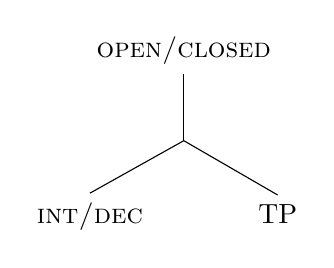
\begin{tikzpicture}[level distance=30pt]
\tikzset{level 1/.style={sibling distance=15pt}}
\tikzset{level 2/.style={sibling distance=35pt}}
\Tree
[. \tsc{open/closed} [ \tsc{int/dec} [.TP ] ] ]
\end{tikzpicture}
\end{center}
\caption{Extended structure of CP proposed by \textcite{farkasroelofsen2017}}
\label{fig:bg:fb2017}
\end{figure}

While the morpho-syntax of a sentence is linked to \tsc{dec/int}, the intonation (rise vs. fall) signals whether C bears the feature [\tsc{open}] or [\tsc{closed}]. Rising declaratives like (\ref{ex:bg:theory:prosody:rd}) would be an ``open declarative,'' with the following structure:

\begin{figure}[H]
\begin{center}
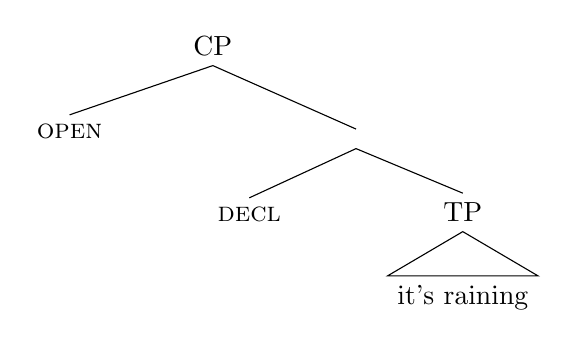
\begin{tikzpicture}
\tikzset{level 1/.style={sibling distance=35pt}}
\tikzset{level 2/.style={sibling distance=35pt}}
\Tree
[. CP 
	[. \tsc{open} ]
	[. \tsc{}
		[. \tsc{decl} ]
		[. TP \edge[roof]; {it's raining} ] 
	]
]
\end{tikzpicture}
\end{center}
\caption{The structure of rising declaratives, adapted from \textcite{farkasroelofsen2017}}
\label{fig:bg:fb2017rd}
\end{figure}

So for \textcite{farkasroelofsen2017}, the clause type category of rising declaratives is not exactly declarative with [$-$int], and its semantics is even similar to that of the polar interrogatives. But as many have noted, there might be two types of rising declaratives. The one discussed in \textcite{farkasroelofsen2017} is the inquisitive one, but there might an assertive one (\cite{jeong2018, goodhue2021rd}), as shown in (\ref{ex:engcl:annt:rd:a}):

\bex{ex:engcl:annt:rd-cont}
\bxl
\label{ex:engcl:annt:rd:q}
\tit{S and A are on their way to a birthday party for the daughter of A’s friend. They stop at a store to get a birthday card. As they are both scanning the display for a card for the correct age, S is trying to remember how old the girl has just turned, and he thinks he remembers A telling him that she just turned nine, but he wants to confirm it.}\\
\tbf{S: She’s nine$\nearrow$}
\ex
\label{ex:engcl:annt:rd:a}
\tit{S is enrolling his daughter in a summer camp program with the camp organizer A.}\\
S: I want to sign her up for Spanish classes in the mornings, and rock climbing in the afternoons.\\
A: Okay, there are limited places in each activity based on age group, and some of the age groups have already filled up for rock climbing. How old is your daughter?\\
\tbf{S: She’s nine$\nearrow$}
\exl
\hspace*{\fill}\hfill ex. (12-13), \cite[p.955]{goodhue2021rd}
\eex

In (\ref{ex:engcl:annt:rd:q}), the speaker uses the utterance to elicit a confirmation from the addressee regarding the age of the birthday girl, so the main goal is to solicit responses, similar to that of questions. But in (\ref{ex:engcl:annt:rd:a}), the speaker uses the rising declarative to answer the question raised by the addressee, proposing to add the proposition \tit{she's nine} to the common ground of the conversation. Even though there is an additional effect associated with the utterance (something to the effect of ``Is there still room in the 9-year-old’s rock climbing group?''), this additional effect is not the main goal of the utterance. \footnote{There is another incredulous use of rising declarative, but the two uses mentioned here are more relevant for the current discussion on the speech act of rising declaratives, as most agree that incredulous rising declarative is also ``inquisitive'', same as (\ref{ex:engcl:annt:rd:q}).} Thus, we might not need to assume an interrogative semantics for rising declaratives.\footnote{Note that if we paraphrase (\ref{ex:engcl:annt:rd:a}), we cannot use \tit{wonder} either:

\bex{ex:bg:theory:prosody:rd-prepose2}
\tit{S is looking a flyer looking for Spanish speakers.}\\
``I speak Ladino $\nearrow$," S thinks/$^{??}$ S wonders.
\eex
 
This suggests that the conclusion we can draw from the test with pre-posed embedded clause might need to be re-examined.}  As \textcite{goodhue2021rd} demonstrates, it is possible to give a unified account for these two uses of rising declaratives without assuming a separate layer of clause type markers. Therefore, in this dissertation, I assume that rising declaratives are declaratives with [$-$int] in $C^{0}$. Since nobody has argued that interrogatives with falling intonation should be classified as having a different clause type as interrogatives with rising intonation, I assume that intonation can modify the conventional effects of a clause (and hence the speech act expressed), and maybe even serve as a cue for identifying clause types, but [\textpm int] does not manipulate intonation the same way it manipulates, say, the word order of subject and auxiliary.

%%BUt going beyond English, there are language that use prosody to disnguish clause types...European portugese...French


\section{Acquisition of speech acts and clause types}
\label{sec:bg:acq}
\subsection{Early communicative abilities}
\label{sec:bg:acq:pre}
As mentioned in the previous chapter, it would be very useful for learners if they could rely on speech act information to learn how clause types are expressed in their language. Speech acts are, unfortunately, not directly observable, but there may be cues accessible to learners that are broadly indicative of speech act. One good candidate are cues for communicative intent.
Previous studies have shown that infants are sensitive to %can recognize
communicative intentions even in their first months of life, and they can distinguish signals for communication, such as eye contact, intentional pointing, and speech, from non-communicative signals. Infants tend to follow the gaze of their interactive partner. Newborn babies already show rudimentary form of gaze following (\cite{farroni2004gaze}); as young as 3 months of age, infants seem to automatically orient to gaze cues, as they could shift gaze fast with adult’s gaze direction (\cite{hood1998gaze}); 6-month-olds follow gazes that are communicative, such as adults' directly gazing at an object (\cite{gredeback2008gaze}), or being greeted (e.g. ``Hello!'') in infant-directed speech (\cite{senju2008gaze}). Human infants, but not chimpanzees, understand pointing as intentional (\cite{pika2006point, povinelli1997point,morissette1995joint}); 9-month-olds remember different aspect about an object depending on whether the object is presented in a communicative (such as pointing) vs.\ non-communicative scenario (\cite{yoon2008intent}); 12-month-olds not only follow the direction of pointing, but also infer that the pointing is to indicate information such as where a toy is hidden in hide-and-seek games (\cite{behne2005hide,behne2012point}). Starting from six months old, infants can readily interpret speech as indicating communicative intentions, as oppose to other vocalizations like coughing (\cite{vouloumanos2014intent}).

Of course, merely recognizing an act \emph{as communicative} is not the same as distinguishing speech acts -- beyond the recognition that there is communication, one needs to infer the function of the communication to approach speech act recognition.
But besides recognizing a signal as communicative, infants can attribute simple goals and desires to an agent, and use shared experience to infer their goals. By 9 months old, infants can recognize an agent's goal of reaching for an object (\cite{woodward1998goal,baldwin2001goal});\footnote{But studies show that still have difficulty with the avoidance type of goals until 14 months old (\cite{feiman2015goals}).} 14-month-olds can distinguish actions that are intentional and ones that are accidental, and only imitate actions that are intentional (\cite{carpenter1998intent,sakkalou2013goal}), and if things go wrong, they offer to help achieve others' goals (\cite{warneken2007goalrecog}); they could use shared experience such as cleaning up toys to interpret an agent's pointing as putting away the pointed object away, and would not attribute this goal to an agent who don't have the shared experience (\cite{liebal2009goal}).

Relatedly, it seems that infants have some understanding of other people's desires and beliefs, attitudes that frequently associated with the speech acts of assertions, questions, and requests. For example, 9-months-old can distinguish whether someone is unwilling or unable to hand them a toy (\cite{behne2005goal}); 12-month-olds can use eye gaze and positive affect to infer which object an agent is going to reach (\cite{phillips2002gaze}), and by 18 months old, infants use positive affect alone to infer which object the agent prefers, even if the preference is different from their own (\cite{repacholi1997desire}). Around 12-month-olds use pointing not to merely direct others' attention, but to request others to share information (\cite{kovacs2014request}); 13-month-olds seek information to clarify ambiguous situations (\cite{vaish2011request}); by 18 months old, infants are shown to be able to attribute beliefs to other people (\cite{onishi2005tom,surian2007tom,song2008earlytom,song2008false, scott2009tom,perner2012earlytom}, see \cite{scott2017review} for a recent review). 18-month-olds could use common ground knowledge shared with an agent to infer whether the agent is requesting an action with an object (e.g. open the door with the key) or simply playing with the object (\cite{schulze2015indirect}).%16-mo use pointing to solicit informaiton (\cite{begus2012point}); 2-year-olds are shown to use what others know when requesting help (\cite{oneill1996knowledge}). 
 


Infants also have some understanding of the norms of conversations. For example, from early on, they understand that conversations take turns. Longitudinal studies with 3 to 5-month-olds show that the overlap between infants' vocalization and parents' speech gradually decrease (\cite{hilbrink2013turn3mo}), and the rhythm of their vocalization starts to mimic the structure of a conversation, as they wait for parents to finish their turn (\cite{hilbrink2013turn,hilbrink2015,casillas2016corpus}); they also use turn transition points (e.g. questions) to cast predicative eye gaze to the next speaker (\cite{casillas2017turn}).

 
 %\textcite{} finds that 
 
In sum, this body of work suggests that by 18 months old, the communicative abilities needed to acquire the distinctions between speech acts and map them to clause types are in place. In the next section, we will see that indeed by this age, infants seem to figured out the major speech acts and are able to link them to their canonical clause types.



\subsection{Early knowledge of clause types and speech acts} \label{sec:bg:acq:spcl}

Previous studies show that children seem to have knowledge about clause types and the associated speech acts (in particular interrogatives and questions) from as early as 18 months old. 

Using corpus data, many studies show that infants can use one- and two-word utterances to express a variety of intentions that can be interpreted as \aqrs{} (\cite{bateson1975,bates1976language,ninio1994} among others); English-speaking children start producing interrogatives around 20 months starting with polar and \twh-interrogatives (\citealt{tyack1977, stromswold1995, rowland2003cdswh}). From the comprehension side, results from corpus studies on parent-child interactions show that children begin to respond to parents’ questions, especially \tit{who, what, where} questions, appropriately around one and a half years old (\citealt{ervintripp1978, steffensen1978, shatz1978comprehension, shatz1978communicative, berningergarvey1981, shatzmccloskey1984, clark2015turn, moradlou2020} among others). 





Results from experimental studies show that around 12 months, English-speaking infants show sensitivity to differences in word order (\citealt{geffenmintz2015wordorder}) associated with declaratives and polar interrogatives respectively. Data from preferential looking tasks show that already at 15 months old, infants look at the objects corresponding to the answers of \twh-interrogatives (\citealt{seidl2003wh, gagliardi2016wh, perkins2020filler}), though their success might not necessarily reflect knowledge of \twh-interrogatives, as they might be relying on their knowledge of verb argument structure in the task (\citealt{perkins2019}). 

By 18 months old, infants seem to be able to distinguish questions from assertions, and use this distinction to infer the epistemic state of the speaker. \textcite{luchkina2018infant} test how well 18-month-olds’ learn labels of novel objects from speakers who made statements about familiar objects (e.g., \tit{This is a star}) and from speakers who asked questions (e.g., \tit{Is this a star?}). They find that even though both types of speakers make statements when labeling novel objects during the test phase, 18-month-olds only learn novel labels from the speaker who made statements during the familiarization phase, but not from the question-askers. This result suggests that 18-month-olds can differentiate questions from statements, and further use this distinction to infer that question-askers might be less reliable information source than statement-makers. 

\textcite{marshmallowqueen} demonstrate that 18-month-olds can associate interrogative syntax with the speech act of questioning with the preferential looking paradigm. In the experiment, infants watch a video of two puppets cheering a mechanical arm for delivering cookies into a box. During the test phase, one of the puppet leaves the scene while the cookie is being delivered, and is thus ignorant of whether there is a cookie in the box. Then participants either hear a polar interrogative \tit{is there a cookie in the box?} or a declarative \tit{there's a cookie in the box!} that could be uttered by either puppet. They find that at 18 months old, infants look more at the ignorant puppet when hearing the polar interrogative, suggesting that they understand the polar interrogative as a question uttered by the ignorant puppet.

\textcite{casillas2017turn} tap into children's knowledge of turn-taking to see if children differentiate questions from other types of speech acts. They measure how often children switch their gaze to track the upcoming speaker. Since questions are turn-transitioning points where a switch in speaker is mostly likely to happen, if children can identify questions, they should switch gazes to the upcoming speaker more often after questions. In the experiment, children are shown videos of a conversation between two puppets in one of four conditions: with normal speech, with words only (filtering out prosodic cues), with prosody, or with no speech. They find that even at 1 years old, children are faster at switching their gaze to the addressee after questions than non-questions in general. Breaking down the different cues to questions, they find that in the word-only condition, even 1-year-olds switch their gaze to the upcoming speaker more often after questions, but in the prosody-only condition, 5-year-olds still are at chance distinguishing questions from non-quesitons. These results suggest that 1-year-olds might be able to use the morpho-syntactic properties of interrogatives to infer questions. Similar results are replicated with 2.5-year-olds by \textcite{lammertink2015turn}.


As for imperatives and commands, \textcite{who?} show that even in the ``telegraphic speech'' phase (15-30 months old), children respond appropriately to imperatives as commands. \textcite{orfitellihyams2012subj} show that 2.6-year-olds can use the presence/absence of verb morphology to tell whether the sentence is a pro-drop declarative or an imperative. 

Previous studies on questions in speech to children suggest that parents use questions in many different ways (\citealt{holzman1972, shatz1979, tamir1980, yu2019pedagogical}). In particular, compared to questions in adult-directed speech (\citealt{stivers2010}), parents tend to use question as a pedagogical strategy. \citealt{zaitsu2020} investigates the frequencies of the three basic clause types and the corresponding speech acts in speech to children between the age 1 to 3 from the Providence corpus (\citealt{ProvidenceCorpus}) of CHILDES (\citealt{CHILDES}). The results show a relatively robust association of declaratives with assertions, but less so of interrogatives and questions due to questions being often asked via rising declaratives, and requests made with interrogatives. %%still a little odd



Going beyond English, Mandarin-speaking children are observed to produce \ma-interrogatives, A-not-A interrogatives, and \twh-interrogatives around 2 years old (\citealt{miao1986acq, miao1992, lee1989acq, litang1991int, lichen1997compprod, lichen1997comp, fan2012, lijingwong2017}). Experimental studies testing children’s comprehension suggest that Mandarin-children have adult-like interpretation of \twh-interrogatives around 3 years (\citealt{fahn2003acq}), but not of polar interrogatives (\citealt{moradlou2020}). 

In our prior work, we find that Mandarin-speaking three-year-olds have adult-like interpretations of \twh-phrases, of both the interrogative and the non-interrogative uses. Our first experiment tested sentences like (\ref{bg-acq:dou}) and (\ref{bg-acq:ba}), where the interrogative and non-interrogative interpretation of the \twh-phrase is disambiguated by morpho-syntactic information (the presence/absence of the particle \dou{}):

	
\bex{bg-acq:dou}
\gll Xiaoyang 	\tun{shenme} 	\tit{dou} 	fangzai 	xiangzili 	le.\\
Lamb	what	\Dou{}	put 	box		\Asp{}\\
``Lamb put everything in the box.''
\eex
\bex{bg-acq:ba}
\gll Xiaoyang	\tit{ba} \tun{shenme} 	fangzai 	xiangzili 	le\\
	Lamb	\tsc{ba}	what	put	box		\Asp{}\\
	``What did Lamb put in the box?''
\eex


Our results show that children, like adults, respond with ``yes/no'' to sentences like (\ref{bg-acq:dou}) but not to (\ref{bg-acq:ba}), suggesting that they can treat the former as an assertion and the latter as a \twh-question. In a second experiment, we present 3-year-olds and adults with negated sentences like (\ref{bg-acq:negwh}) where the sentence is ambiguous between an assertion and a \twh-question. In this case, the two interpretations are disambiguated by prosodic cues: assigning prosodic prominence on \tit{shenme} gives rise to a \twh-question interpretation, and without prosodic prominence, the sentence is an assertion. Our results again show that 3-year-olds, like adults, can access both interpretations of the sentence.


\bex{bg-acq:negwh}
\gll Xiaoyang mei	fang	\tun{shenme} shuiguo zai	xiangzili\\
Lamb \Neg{}	put	what		fruit		in	box\\
\trans a. ``What fruit didn't Lamb put in the box?''\\
b.	``Lamb didn't put any fruits in the box.''
\eex

\section{Summary}
In this chapter, I reviewed the different theories on clause type and speech act. I also show that regardless of the theoretical stance, people agree on the three major clause types and their corresponding three major speech acts. 

Additionally, results from previous studies show that by by 18 months old, infants seem to have figured out the major clause types and speech acts, and the link in-between. These studies give us a developmental window for our models, namely that our models need to take into account what infants know around 18 months old, to simulate how they figured out clause types and speech acts at this age. In the next chapter, I delve into the problem of how 18-month-olds figure out clause types.


%In summary, children might face many challenges when learning interrogatives and their mapping to questions: English-speaking children should identify word order as a cue for interrogativity, but this information might be buried under many exceptions; Mandarin-speaking children should identify the markers for interrogativity (e.g.~\twh{}) despite some of these markers occurring in non-interrogative environments. Moreover, in both languages, children have to recognize the link between interrogativity and questionhood, which might be masked by exceptions in their input. So, how do children acquire interrogatives and their relationship to questions? In the next section, we will see that despite the noisiness of the input data, there is evidence suggesting that children nevertheless have adult-like understanding of interrogatives, questions, and their relationship at around three years old if not younger. 



 %\cite{evans2014ids} \cite{bernicot1987imp}


\chapter{Learning to identify clause types in English}
\label{chap:eng-cl}


As discussed in the previous chapters, cross-linguistically we see three major clause types, declaratives, interrogatives, and imperatives, dedicated to three main speech acts, assertions, questions, and commands/requests. We also see in Chapter~\ref{chap:background}, by 18 months old, infants seem to have figured out the differences among these clauses and how they are associated with their canonical functions.  To gain this ability, they must have solved a number of learning problems. Specifically, as discussed in Chapter~\ref{chap:introduction}, learners need to solve the \tbf{clustering problem}, i.e. clustering clauses in the right three categories, and the \tbf{labeling problem}, i.e. linking each category to its function. 

Given that infants's early success at identifying clause types, this chapter investigates how learners solve these problem, especially the clustering problem, by probing the extent to which children need to rely on pragmatic information (i.e., knowing what speech act a given utterance of sentence is conveying). As discussed in Chapter~\ref{chap:introduction}, pragmatic information is essential for solving the labeling problem. The question I ask here, then, is whether pragmatic information is also crucial for solving the clustering problem, as well. Will a learner strictly tracking formal regularities home in on the right three clusters of clauses? Will a learner privy to some speech act information fare better? How much pragmatic information is required? To answer these questions, I compare the performance of two computational models, a \tbf{\distlearner{}} (\dlearnerabbr{}) and a \tbf{\praglearner{}} (\plearnerabbr{}), using data from an annotated dataset I created with parental sentences in the Providence Corpus (\cite{ProvidenceCorpus}).

This rest of the chapter is organized as follows: 
In Section~\ref{sec:engcl:background}, I first briefly introduce the two computational models mentioned above, and how they can help us answer our questions (Section~\ref{sec:engcl:bg:learners}). I then review the formal features of English \diis{} (Section~\ref{sec:engcl:bg:grammar}), setting the stage for discussing the learning of these clause types. But these are features that English employs for clause typing, infants at 18 months old might not be able to perceive all (or the full-fledged version) of these features. To allow our models to best capture 18-month-olds' learning process, we need to look at 18-month-olds' linguistic capacity and knowledge with regard to these features. So in Section~\ref{sec:engcl:bg:assumptions} I briefly go through the linguistic capacities and knowledge of infants before 18 months old with regard to the formal features used for clause typing, which in turn will guide the way these features are coded in the corpus. 

In Section~\ref{sec:engcl:corpus}, I report results from a corpus study on parents' use of different clause types and speech acts, to give a quantitative description of the information present in the input. The annotated dateset result from this corpus study will be used in our modeling experiments.

Section~\ref{sec:engcl:model} details the two computational models for the two learners, \dlearnerabbr{} in Section~\ref{sec:engcl:model:baseline} and \plearnerabbr{} in Section~\ref{sec:engcl:model:pragmatics}, to see if pragmatic information is needed for solving the clustering problem. I then manipulate the ratio of noise in the pragmatic information to see how much pragmatics is needed (Section~\ref{sec:engcl:model:noisy}). Section~\ref{sec:engcl:discussion} concludes the chapter. 


\section{Background}
\label{sec:engcl:background}

\subsection{Two learners} 
\label{sec:engcl:bg:learners}
As mentioned above, the question we set out to answer is whether pragmatic information, specifically, the speech act expressed by the sentence, is necessary for learners to solve the clustering problem and find the right clause type categories. To this end, I build two computational models learning the clustering of clauses, a \text{\distlearner{}} (\dlearnerabbr{}) and a \text{\praglearner{}} (\plearnerabbr{}). Both learners are forms of distributional learning: they track distributions of certain features in their input, and use these observations to infer the underlying categories that gives rise these distributions
(cf. \cite{feldman2013,gagliardi2017modeling,perkins2022vmodel,perkins2019,nguyenwilson2021}; see \cite{pearl2020review} for a recent review). Specifically, these two learners share the same goal of discovering the underlying clustering of sentences in parents' speech, i.e. to infer the abstract clause type categories in English. The difference between them lie in the sources of information they take as input. 

The \tbf{\distlearner{}} (\dlearnerabbr{}) assumes that learners track the statistical distributions of \tit{morpho-syntactic features} present in the surface forms of sentences to infer the abstract clause type category that gives rise to these distributions. This learner serves as our baseline; by looking at its performance, we will be able to see how far syntactic information alone could take a learner in learning clause types. 

The \tbf{\praglearner{}} (\plearnerabbr{}) also tracks the distributions of morpho-syntactic features, but at the same time, it  keeps track of the speech acts expressed by these sentences as well. Thus, it infers clause type categories with information from both syntax and pragmatics. 

Thus, we would be able to answer the question of whether pragmatics is crucial for the clustering problem by comparing the performance of these two learners: if pragmatic information indeed helps the learner, not only with labeling but also with clustering, we would see \plearnerabbr{} outperforms \dlearnerabbr. Additionally, if \plearnerabbr{} indeed performs better, we can manipulate the ratio of noise in the pragmatic information that \plearnerabbr{} receives, to see how much pragmatics learners need to solve the clustering problem. 


The success of these two learners depend on the specific features we feed into the models. In Chapter~\ref{chap:background}, we have talked about speech acts extensively, but the morpho-syntactic features for clause typing differ from language to language. In the next section, we will go through the specific morpho-syntactic features that English employs for clause typing, to set the stage for our discussion of the learning of clause types. 


\subsection{Clause types in English} \label{sec:engcl:bg:grammar}

Generally, clauses in English are marked by the presence of verbs (\ref{ex:engcl:fragments}a). Sentences without verbs are often classified as fragments (\cite{sz1985speechact}), as in (\ref{ex:engcl:fragments}b):
\bex{ex:engcl:fragments}
\bxl{}
Mary hugged Ann.
\ex
Mary!
\exl
\eex

In this section, we will go over the properties of thethree major types of clauses, \diis{}, in English. 

As many have observed, the declarative clause in English tend to be ``unmarked'' (sometimes analyzed as $C$ carrying a [-int] feature) , and interrogatives and imperatives are sometimes analyzed as being the results of operations on declaratives (\cite{sz1985speechact, chomsky1957,chomsky1995minimalist, akmajian1984clausetype, platzack1997imp,rizzi1997} among many others). For example, rule $T_{q}$ in \textcite{chomsky1957} transforms a declarative sentence to an interrogative by switching the order between the subject constituent and the auxiliary constituent:
\bex{ex:engcl:chomsky:tq} 
\bxl
Structural analysis: $ \left\{\begin{array}{l}
NP-C-V \ldots\\
NP-C+M-\ldots\\ 
NP-C+\textit{have}-\ldots\\ 
NP-C+\textit{be}-\ldots 
\end{array} \right \}
$
\ex Structural change: $X_{1} - X_{2} - X_{3} \rightarrow X_{2} - X_{1} - X_{3} $
\hfill \textcite[p.112]{chomsky1957}
\exl
\eex

This rule illustrates the hallmark of interrogativity, subject-auxiliary inversion: for sentences that can be analyzed as having a subject NP followed by an auxiliary ($C$ in the structural analysis rule), apply the structural change transformation to move the auxiliary\footnote{In the case of null auxiliary (the first case), the affix rule $\#Af\rightarrow \# do+ Af$ applies to supply do-support.} in front of the subject. This trademark of [+int] value of English $C$ can be seen in polar interrogatives like  (\ref{ex:engcl:subjaux}a) and \twh-interrogatives like (\ref{ex:engcl:subjaux}b). 

\bex{ex:engcl:subjaux}
\bxl{}
Can Mary hug Ann?\hfill polar interrogative
\ex
Who can Mary hug? \hfill \twh-
interrogative
\exl
\eex


However, this association of word order and interrogativity has many exceptions. For example, in subject \twh-interrogative sentences like (\ref{ex:engcl:int-exceptions}a) and sentences with embedded interrogatives (\ref{ex:engcl:int-exceptions}b-c), the interrogative takes the same word order as a declarative. 

\bex{ex:engcl:int-exceptions}
\bxl{}
Who can hug Ann? \hfill subject \twh-interrogative
\ex
Mary wonders \tun{who Ann can hug.} \hfill embedded \twh-interrogative
\ex 
Mary wonders \tun{whether Ann can hug Sue.} \hfill embedded polar interrogative
\exl
\eex

As discussed in Chapter~\ref{chap:introduction}, these cases might be a problem for learners, as they obscure the mapping between the subject-auxiliary inversion rule and [+int]. While the presence of \twh-phrases in (\ref{ex:engcl:int-exceptions}a-b), and complementizer \tit{whether} (\ref{ex:engcl:int-exceptions}c) in these sentences are also cues for [+int], these features suffer the same problem. For example, free relative sentences (\ref{ex:engcl:whexceptions}) also appears with a clause-initial \twh-phrase, but the $C$ head this \twh-clause has the feature [-int] (\cite{bresnan1978free, caponigro2003free}):

\bex{ex:engcl:whexceptions}
Mary ate \tun{what Ann cooked.} \hfill Free relative sentences
\eex

%Mary claims that she ate what?
%in-situ \twh-questions,\footnote{We adopt the analysis given by \textcite{bobaljik2015echo} here that this type of \twh-questions are in fact declaratives with [-int] in their $C$. One of the reasons for this analysis is that these types of clauses cannot be selected by rogative verbs like \tit{wonder}:
%\begin{xlisti}
%\exi{(i)} *I wonders I should put this stuff where. \hfill (ex. (8b), \cite[p.18]{bobaljik2015echo})
%\end{xlisti}
%}


Meanwhile, some declaratives exhibit subject-auxiliary inversion as well, such as Negative Inversion sentences like (\ref{ex:engcl:neginvert}): these sentence are generally considered declaratives, but the auxiliary \tit{would} precedes the subjects in both.

\bex{ex:engcl:neginvert}
\bxl{}
Never in her life would Mary eat tripe.
\ex
Under no condition would Mary eat tripe.
\exl
\eex

These might be cases where the speech act information might be able to help, as identifying the utterance as making an assertion might help the learner avoid making the generalization that [-int] also triggers subject-auxiliary inversion. 

Imperatives (some analyzed as $C$ having the feature [imp], \cite{platzack1997imp}) in English typically use bare verb stem. In most cases, subjects are missing (\ref{ex:engcl:imp}a), but sometimes there are subjects expressing the addressee (\ref{ex:engcl:imp}b).

\bex{ex:engcl:imp}
\bxl{}
Be quiet!
\ex You be quiet!
\exl
\eex


In sum, declaratives ([-int] feature in $C$) in English are the unmarked clause type; interrogatives ([+int] in $C$) are associated with subject-auxiliary inversion, presence of clause-initial \twh-phrases, presence of complementizer \tit{whether}; imperatives ([imp] in $C$) are marked by using verb stems, and absence of sentential subjects or have second person pronouns as subjects. So to successfully infer the clause type categories, learners have to pay attention to morpho-syntactic features like the presence or absence of the sentential subject, the form of the verb, the position of the auxiliary, the presence or absence of \twh-phrases in clause-initial position, the choice of complementizers in the surface form of sentences. Table~\ref{tab:engcl:grammar} summaries the morpho-syntactic features and their associated clause types:


\begin{table}[H]
    \centering
\begin{tabular}{l|l } 
\hline
Feature  & Examples\\ 
\hline \hline
\multirow{2}{*}{$\pm$ \tsc{verb} }&
($+$) \tbf{Find} Elmo! \hfill Clause\\

&($-$) Elmo! \hfill Fragment
\\ 
\hline
\multirow{2}{*}{\tsc{$\pm$ subject} }&
($+$) \tbf{I}'ll take it. \hfill [$-$imp]\\

&($-$) Take it. \hfill [+imp]
\\
\hline
\multirow{2}{*}{\tsc{$\pm$ verb suffix} }&
($+$) Nobody feel\tbf{s} good huh? \hfill [$-$imp] \\

&($-$) Find Elmo! \hfill [+imp]
\\ 
\hline
\multirow{2}{*}{\tsc{$\pm$ subj-aux inversion} } & 
($+$) \tbf{Can you} find the ladybug? \hfill [+int]\\

&($-$) I can take it. \hfill [$-$int]
\\ 
\hline
\multirow{2}{*}{\tsc{$\pm$ sentence-initial \twh{} }} & 
($+$) \tbf{What} did you find? \hfill [+int]\\

&($-$) I found it. \hfill [$-$int] \\
\hline
\multirow{2}{*}{\tsc{complementizer} } & 
($+$) I know \tbf{whether} it's wrong. \hfill [+int]\\

&($-$) I know that it's wrong.\hfill [$-$int]
\\
\hline
\end{tabular}

\caption{Morph-syntactic features and their associated clause types}
\label{tab:engcl:grammar}

\end{table}

Of course, as we have discussed, many features do not have a one-to-one mapping with the abstract clause type categories. So apart from using the right features to cluster clauses, learners also need to avoid making certain generalizations about a feature in some cases (e.g. avoid associating subject-auxiliary inversion with declaratives upon seeing Negative Inversion sentences).  
 
While these features are significant in the grammar, it's likely that not all of these features (or the full-fledged version of these features) can be perceived by 18-month-olds. If we want to model how 18-month-olds learn clause types, the way we code these formal features in our corpus (which serves as the input to our models) has to be sensitive to their linguistic knowledge, and what they are able to perceive at the relevant age. In the next section, I will review what linguistic knowledge and capacities children have around 18th months with regard to these formal features. 

\subsection{Linguistic knowledge and capacities of 18-month-olds}
\label{sec:engcl:bg:assumptions}

Generally, infants have been shown to track distributional properties of various kinds, and 18-month-olds can perceive many grammatical features. How much do they know about the ones that associated with English \diis{} (Table~\ref{tab:engcl:grammar})? In this section, I'll briefly review 18-months-olds' capability regarding the features reviewed in the last section, and relatedly, how we code these features in our corpus. % These features are included to give the \distlearner{} the best chance of succeeding. 

\tsc{$\pm$ Verbs:} By 18 months, infants can recognize whether there is a verb in a sentence. They can use the frequent frames (e.g. adjacency to function words like auxiliaries, pronouns, or have affixes) associated with verbs to categorize a novel word as a verb (\cite{echols2004verb, mintz2006verb,peterson2006aux,soderstrom2007sv, lidzoritaomaki2012, shi2014functional, helidz2017verb} among many others), suggesting that they have knowledge of verbs, and frequent verb frames. 

\tsc{$\pm$ Verb suffixes:} Around this age, infants can recognize some morphological markings on the verb.  As early as 6 months old, English-learning infants seem to be able to segment \tit{-s, -ed, -ing} from a nonce verb (\cite{kimmegha2016morph}). 15-month-olds can segment English verbal suffix \tit{-ing} from a word, but do not do so with pseudo-suffixes (\cite{mintz2013segmentation}); 18-month-olds can distinguish well-formed auxiliary-affix dependencies (e.g. \tit{is...-ing}) vs. an ill-formed ones (e.g. \tit{can...-ing}, \cite{santelmann1998morph}). Thus, we can assume that 18-month-olds can tell whether verb suffixes are present in a sentence.

\tsc{$\pm$ Subject:} Studies have shown that infants have some knowledge about subjecthood by 18 months old.They show sensitivity to subject-verb agreement in English, as they prefer grammatical sentences over ungrammatical sentences with agreement violation (\cite{soderstrom2002agr, soderstrom2007sv, nazzi2011} among others), even if the subject is not immediately adjacent to the verb. They could also use the frame [subject pronoun + verb] to categorize novel words as verbs (\cite{babineau202014func,peterson2006aux, mintz2006verb,shi2014functional} among others). Moreover, and perhaps more important to our study, 12-month-olds are sensitive to the change in word order when the position of the subject and auxiliary is switched (\cite{geffenmintz2015wordorder}). While we do not have evidence that 18-month-olds can use the presence/absence of subjects to tell whether a sentence is imperative or not (\cite{orfitellihyams2012subj} demonstrate that 2.6-year-olds can do it), but we can assume that they can detect whether the subject is present or not.



\tsc{$\pm$ Subj-aux inversion:} By 18 months, infants can recognize whether there is an auxiliary in the sentence, and are sensitive to the relative word order between the auxiliary and the sentential subject. As mentioned above, well before they turn 18 months old, infants can already use preceding auxiliaries to categorize a novel word into the verb category (e.g. \cite{peterson2006aux, mintz2006verb}), suggesting that they understand the relation between auxiliaries and verbs. Additionally, as mentioned above, 12-month-olds can already detect subject-auxiliary inversion (\cite{geffenmintz2015wordorder}); with both word order and prosodic cues, even 7-month-olds are able to detect the difference between polar interrogatives and declaratives (\cite{geffenmintz2011}). We therefore assume that infants are able to detect whether there is an auxiliary in the sentence, and further they are able to detect whether the subject is preceding or following the auxiliary.

\tsc{$\pm$ Sentence-initial \twh{}:} \textcite{perkinslidz2021wh} shows that 18-month-olds, but not younger infants, begin to represent the sentence-initial \tit{which NP} as the head of a long-distance dependency. These results are suggestive, but we do not yet have evidence for the full range of \twh-phrases. In order to be conservative, we do not assume that infants have full-fledged knowledge of \twh{}. However, infants at this age are shown to have the ability to tease apart functional from content words based on their acoustic and phonological properties (\cite{shi1999func,shi2014functional}), and it is reasonable to assume that they could  \twh{s} as functional items (\cite{perkins2019}). Therefore, we will still treat \twh{} as unknown to 18-month-olds, but they are unknown \emph{functional} items (UFI), following \textcite{perkins2019}.\footnote{Note that \textcite{perkins2019} models what happens before 18 months, as her experiment narrows down the developmental window to 18 months old. Moreover, while her experiment only tests \tit{which}, there are some studies suggesting that 18-month-olds can understand \tit{what}, \tit{who}, and \tit{where} . Thus assuming that all \twh-items are unknown functional items might be too conservative. In the future, I plan to see if loosening this assumption (e.g. assume that some \twh-items are known) will boost the performance of the \dlearnerabbr{}.} We can also assume that 18-month-olds can keep track of the position of these UFIs in the sentence, whether they are clause-initial, middle, or end. So they could detect whether is a clause-initial UFI. 

\tsc{Complementizer:} So far, we do not have evidence for infants' knowledge of complementizers at this age, but again they might be able to categorize complementizers as functional items. So these are treated as UFIs as well.\footnote{ Other functional items that we do not have evidence for 18-month-olds include quantifiers, focus particles, or certain conjuntors such as \tit{because}. I assume that these are UFIs as well. } %Similarly, we 


%Table~\ref{} summarises our assumptions about 18-month-olds' knowledge of the set of formal features that associated with clause typing.


%Finally, infants can perceive some features of prosody, and might be able to use some non-clause type-related features to infer speech acts. We will come back to both in Chapter~\ref{chap:eng-sp}.

In summary, apart from clause-initial \twh-phrases (which we assume will be perceived as clause-initial UFIs), 18-month-olds have the formal features relevant for clause typing in English. But how do parents use clause types and speech acts? How serious is the many-to-many mapping problem, between clause type and speech act, and between formal features and clause type? We will address these questions with a corpus study. %The annotated dataset resulted from this study will be used in our computational modeling experiments.

\section{Corpus study}
\label{sec:engcl:corpus}
To understand how infants figure out clause types and speech acts, we first need to establish what kind of information is present in the input. Specifically, we need to know the morpho-syntactic features of parents’ sentences, and in what contexts parents use different speech acts. For example, how available is word order as a cue to interrogativity in English-speaking parents’ speech? Are interrogative sentences associated with similar prosodic features? Do word order and prosodic features jointly correlate with interrogativity? Are there any correlations between the formal properties like syntactic and prosodic features of parents’ interrogative and their functional properties? In this section, I’ll report findings from the corpus study on parental input to English-speaking infants. 


\subsection{Corpus and Methods}
\label{sec:engcl:corpus:methods}
%%%%PAST TENSE
This study used data from the Providence sub-corpora (\cite{ProvidenceCorpus}) from CHILDES (\cite{CHILDES}), which contains conversations between 6 children and parents recorded between 2002-2005 in Providence, RI. We selected this particular corpus because it covers children’s interaction with parents at the critical age that we are interested in ($\leq$ 18 months old). Additionally, it contains transcripts, audio, and video data, providing us with an opportunity to not only look at the morpho-syntax of parents’ sentences, but also their prosodic information, and even parents’ behavior accompanying each utterance. Parent-child interaction data from five typically developing children in this corpus were included in this study: Alex, Lily, Naima, Violet, and William. %For each session, we used the transcript to annotate  

We sampled 500 conversational turns from each session with the annotation schema detailed in the next section. For the clause type and speech act information, each transcript was annotated by two annotators and compared for differences. In cases of disagreement, the two annotators would have a discussion, and if the difference cannot be resolved, a third person would be consulted. To annotate the speech act information, annotators were asked to look at 20 utterances before and 2 utterances after the current utterance in the conversation, as well as consulting the videos for contextual information. For the morpho-syntactic features, initial annotation was generated by a script (\textcolor{red}{url}) using the morphological tagging provided by CHILDES, and then manually corrected. 

In total, we annotated 9147 utterances. We will return to the video and audio part of the annotation process in Chapter~\ref{chap:eng-sp}.




\subsection{Annotation schema}
\label{sec:engcl:corpus:schema}
%As results from our corpus study would serve as input and gold standard for our models, . Our annotation schema is hence designed to capture the syntactic and prosodic features of interrogatives and their uses in the discourse. In this section, we will detail our annotation schema at each level. 
%will be coded by examining the utterance in isolation and thus in the absence of any information about the surrounding discourse. Functional features will be coded based on a combination of discourse information, the audio recordings, and the video recordings, as explained in greater detail in Section 3.2.3.  Two annotators will code the data independently and then compare for reliability. Disagreements will be settled by the two annotators by assessing the data together and, if necessary, consulting a third annotator. If a new feature category is identified as necessary, both coders will again annotate the data independently and compare for reliability. The full annotation schema can be accessed here.

\subsubsection{Clause Type}

All sentences were annotated with clause type information: declarative (\ref{eng-cl:annt:cl}a), interrogative (\ref{eng-cl:annt:cl}b), or imperative (\ref{eng-cl:annt:cl}c). Two other categories were included: Fragment and Ambiguous. In cases where the utterance only contains a noun or an injective without verbs like (\ref{eng-cl:annt:frag}), the utterance was annotated as a Fragment. In some cases, the sentence does not contain enough information to decide the clause type categories, and will thus be labelled as Ambiguous. For example, sentences like (\ref{eng-cl:annt:cl}d) could either be a case of pro-drop from the declarative sentence \tit{you want to get down}, or it could be a case of left-edge ellipsis from the polar interrogative \tit{do you want to get down}. Note that it is in principle possible to distinguish pro-drop from left-edge ellipsis; for example (\ref{eng-cl:annt:disamb}a) has to be a case of left-edge ellipsis from \tit{are you coming}, and (\ref{eng-cl:annt:disamb}b) is a case of pro-drop from \tit{I went to the store yesterday}. As the sentence in (\ref{eng-cl:annt:frag}) does not contain these morphological clues for us to make the distinction, it will be classified as Ambiguous.

\bex{eng-cl:annt:cl}	
Clause type
\bxl
\label{eng-cl:annt:decl}
It’s all twisted. \hfill Declarative
\ex \label{eng-cl:annt:int} What happened?	\hfill Interrogative
\ex \label{eng-cl:annt:imp} Throw it.\hfill Imperative
\ex \label{eng-cl:annt:frag}	Elmo!\hfill	Fragment
\ex \label{eng-cl:annt:amb} Wanna get down?	\hfill Ambiguous
\exl
\eex

\bex{eng-cl:annt:disamb}
\bxl{} You coming?\hfill Left edge ellipsis; interrogative
\ex went to the store yesterday. \hfill	Pro-drop; declarative
\exl
\eex

Interrogatives will be further divided into subcategories as polar, \twh, and disjunctive interrogatives:

\bex{eng-cl:annt:subI}	Sub-types of interrogatives
\bxl{}
Is that a big bird shovel? \hfill	Polar interrogative
\ex	Who is that?\hfill	\twh-interrogative
\ex	Do you want water or juice? \hfill Disjunctive interrogative
\exl
\eex

\subsubsection{Speech Act}

Three major speech acts categories are labelled: assertions, questions, requests/commands:\footnote{The distinction between requests and commands are subtle, and often involves the calculation of the social hierarchy between conversational partners. As parents hold authority over the child, even if the parent intend an utterance to be a request, it could be perceived by the child as a command. Therefore, we do not make a distinction in this study.}

\bex{eng-cl:annt:sp}
\bxl{} It’s all twisted!\hfill	Assertion
\ex Is that the postman?\hfill		Question
\ex Throw it!	\hfill		Request/command
\exl
\eex

As discussed in the last chapter, in many cases, one clause can used to perform both a primary speech act, and a secondary indirect speech act. For this study, we labelled the primary act performed by the utterance. For example, (\ref{eng-cl:annt:indirect}) performs a primary act of questioning and an indirect act of making a request. For these cases, the indirect speech act was annotated.

\bex{eng-cl:annt:indirect}
Can you put that down?
\eex 

\subsubsection{Formal features}

As reviewed in the last section, infants at 18 months old might have knowledge of certain morpho-syntactic features. In particular, infants might have knowledge of the subject of a sentence, its position in the sentence (whether in canonical pre-verbal position or inverted), verbs and various functional elements associated with verbs such as auxiliaries and some verbal morphology. Infants might not have a separate category for all the \twh-items, but they might be able to still classify them as functional elements, as they may know the distinction between functional and content elements. We therefore put \twh-items, quantifiers, connectives (except for \tit{and}), and focus particles in one category ``unknown functional item (UFI),'' and we annotated its position in a sentence: sentence initial, sentence-medial but before the verb, or after the verb. Each sentence was annotated with whether or not a specific feature is present. Table~\ref{tab:eng-cl:formal-schema} summarizes the features we annotated and their examples.  


\begin{table}[H]
    \centering
\begin{tabular}{r|l } 
\hline
Feature Name & Examples\\ 
\hline \hline
\multirow{2}{*}{Subject} & 
($+$) \tbf{I}'ll take it.\\
&($-$) Take it. \hfill
\\
\hline
\multirow{2}{*}{Verb} & 
($+$) \tbf{Find} Elmo! \\

&($-$) Elmo! 
\\ 
\hline
\multirow{2}{*}{Verb Morphology} & 
($+$) Nobody feel\tbf{s} good huh?\\

&($-$) Find Elmo! 
\\ 
\hline
\multirow{2}{*}{Auxilary} & 
($+$) \tbf{Can} you find it? \\

& ($-$) I found it! 
\\ 
\hline
\multirow{2}{*}{Subject-auxiliary inversion} & 
($+$) \tbf{Can you} find the ladybug?\\ %\hfill \tcb{Interrogative}

&($-$) I can take it. %\hfill\tcr{Declarative}
\\ 
\hline
\multirow{2}{*}{Sentence-initial UFI}& 
($+$) \tbf{What} did you find?\\ %\hfill \tcb{Interrogative}

&($-$) I can take it.\\
\hline
\multirow{2}{*}{Pre-verbal UFI}&
($+$) Raccoon \tbf{only} comes out at night.\\

&($-$) I can take it.\\
\hline
\multirow{2}{*}{Post-verbal UFI} & 
($+$) I know \tbf{what}'s wrong.\\

&($-$ I know you can do it.
\\
\hline
\end{tabular}

\caption{Formal features and their examples included in the corpus study}
\label{tab:eng-cl:formal-schema}

\end{table}





\subsection{Results}
\label{sec:engcl:corpus:results}


\subsubsection{Overview}
With the schema given above, an annotated dataset consisted of 9047 utterances was created. As we are primarily interested in the form and function of parents' sentences in this chapter, we excluded children's utterances and uninterpretable utterances from the dataset (as children's vocalization might change the pragmatics of the conversation, we will return to them in Chapter~\ref{chap:eng-sp}). Overall, 7039 utterances were analyzed.  Figure~\ref{fig:real-cldist} shows the distribution of clause types in the dataset. Declarative clauses are the most frequent clause type, followed by interrogatives and imperatives. 


\begin{figure}[H]
    \centering
    \includegraphics[width=0.7\textwidth]{figures/real-cldist.jpg}
    \caption{Distribution of clause types}
    \label{fig:real-cldist}
\end{figure}


Zooming in on interrogatives, \twh-interrogatives are more frequent than polar interrogatives; only 2 cases of disjunctive interrogatives were found in the corpus. Figure~\ref{fig:real-subI} shows the distribution of the subcategories of interrogatives. 

\begin{figure}[H]
    \centering
    \includegraphics[width=0.7\textwidth]{figures/real-subI.jpg}
    \caption{Subcategories of interrogatives}
    \label{fig:real-subI}
\end{figure}


As shown in Figure~\ref{fig:real-clsp} and \ref{fig:real-spcl}, the mapping between speech acts and clause types are in fact quite straightforward. The majority of declaratives are used to express assertive force; the majority of interrogatives are used to express question force; and the majority of imperatives are used to express command/request force. 

\begin{figure}[H]
    \centering
    \includegraphics[width=0.7\textwidth]{figures/real-clsp.jpg}
    \caption{The speech acts performed by each clause type in parents' speech}
    \label{fig:real-clsp}
\end{figure}

Conversely, as shown in Figure~\ref{fig:real-spcl}, the majority of assertions are expressed with declaratives, questions with interrogatives, and requests with imperatives.

\begin{figure}[H]
    \centering
    \includegraphics[width=0.7\textwidth]{figures/real-spcl.jpg}
    \caption{The clause type used to express each speech act in parents' speech}
    \label{fig:real-spcl}
\end{figure}


The few cases of mismatches seem to show systematicity as well. For example, declarative and interrogative sentences used for requests/commands tend to have modals, attitude verbs, or future morphology in the sentence:

\bex{eng-cl:dec-req}
\bxl{}	I need you to help me.		\hfill	Mother of William, Session 010605
\ex	Can you say hi?				\hfill	Mother of Lily, Session: 010117
\ex	(previous utterance: I'm gonna do some work.)\\
And you’re gonna do some coloring.\hfill		Mother of Violet, Session: 010407
\ex  Are you gonna read to Mommy?	\hfill	Mother of Lily, Session 010102
\exl
\eex 

Declarative and imperative sentences used as questions all are predominantly marked with final rise intonation. We will return to the prosodic features of each clause type in Chapter~\ref{chap:eng-sp}.

%, as in (\ref{eng-cl:dec-rise}a-b), or have embedded interrogatives (\ref{eng-cl:dec-rise}c):
\begin{comment}
\bex{eng-cl:dec-rise}
\bxl{}
Try this again?			\hfill Mother of William, Session 010605
\ex Oh , you don't wanna play with this ? \hfill	Mother of Naima, Session 001126
\ex Tell Mommy what it says. \hfill Mother of Alex, Session 010427 
\exl
\eex

\end{comment}

\begin{figure}[H]
    \centering
    \includegraphics[width=0.7\textwidth]{figures/real-subIsp.jpg}
    \caption{The speech act expressed by different subcategories of interrogatives}
    \label{fig:real-subIsp}
\end{figure}




Turning to the speech acts of these interrogatives, Figure~\ref{fig:real-subIsp} shows the proportion of speech acts that polar and \twh-interrogatives expressed. The only two examples of disjunctive interrogatives were used both as questions, and thus not graphed in the figure. Polar interrogatives were used to express speech acts than \twh-interrogatives: around 18\% of polar interrogatives were used to indirectly raise requests like in (xx), or indirectly making an assertion like in (xx):

\bex{eng-cl:int-asst}
Polar-interrogatives as assertions:
\bxl{}
Doesn’t he have sharp teeth?	\hfill	Mother of Lily, Session: 010611
\exl
\eex

Few \twh-interrogatives were used as non-question. We found 4 cases of \twh-interrogatives used to indirectly make a request (\ref{eng-cl:wh-req}), and indirectly making assertions by way of asking rhetorical questions (\ref{eng-cl:wh-asst}):\footnote{We did also find sentences with \tit{how about/what about} (see Rawlins and Bledin 2021), but the majority of these sentences do not come with a verb and were considered fragments (\ref{eng-cl:howabout-frag}). But we also found one case of \tit{how about} interrogative with a verb (\ref{eng-cl:howabout-int}), and the primary intention of the utterance is to make a request. 

\begin{xlisti}
\ex \label{eng-cl:howabout-frag} How about this one?	\hfill	Mother of Alex Session 010512
\ex \label{eng-cl:howabout-int} How about we do these babies. \hfill	Mother of Lily, Session 010102
\end{xlisti}
}


\bex{eng-cl:wh-req}
\twh-interrogatives as requests
\bxl{}
Why don’t you turn around.	\hfill Mother of William, Session 010619
\exl
\eex
\bex{eng-cl:wh-asst}
\twh-interrogatives as assertions
\bxl{}
Who doesn’t love cheese?\hfill	Mother of Lily, Session: 010117
\ex Why are there no pens in this family?\hfill	Mother of Violet, Session: 010407
\exl
\eex




\subsubsection{Morpho-syntactic features}
\label{sec:eng-cl:corpus:formal}
We now turn to the question of how parents use each clause type, namely the formal features of each clause type. We therefore exclude fragment utterances that only contain a noun (\tit{Birdie!}), interjective (\tit{Oh}). In total, 3923 sentences were included in the analysis.

The distribution of the morpho-syntactic features listed in Table~\ref{tab:eng-cl:formal-schema} across different clause types is shown in Figure~\ref{fig:real-syncluster}. The x-axis of the figure represents the counts of sentences, and the eight morpho-syntactic features are listed along the y-axis. Each graph is split in the middle: to the left of the line, bars with darker colors represent the counts of declarative, interrogative, or imperative sentences with this specific feature, and to the right, bars with lighter colors represents the number of sentences without this feature. 





\begin{figure}[H]
    \centering
    \includegraphics[width=1\textwidth]{figures/real-syncluster.jpg}
    \caption{The number of sentences with/without certain formal features in each clause type; darker color represents the number of sentences with this feature }
    \label{fig:real-syncluster}
\end{figure}

We can see that parents use the clause types rather systematically: the majority of declaratives and interrogatives are marked by the presence of subjects, as opposed to imperatives; the majority of interrogatives are marked by subjects following the auxiliary or the main verb, contrary to imperatives and declaratives; verbs in imperatives are not marked by having morphological marking on the main predicate. 

Three logistic regression models with each of the clause type as the dependent variable and the 8 morpho-syntactic features (the presence/absence of verbs and unknown functional item at preverbal position were excluded due to extremely low variance) as independent variables were performed, and the results are summarized in Table~\ref{tab:engcl:real-synstats}:


\begin{table}[H]
\begin{center}
\begin{tabular}{r|l|l|l}
\hline
 & Declaratives   & Interrogatives   & Imperatives \\
 & $\beta$  & $\beta$  & $\beta$ \\
 \hline\hline
constant & -1.7*** & -4.91*** & 1.21*** \\
\hline
Subject & 3.35*** & 1.08*** & -4.61*** \\
\hline
Verb Morphology & 1.01*** & 0.21  & -2.02*** \\
\hline
Auxiliary & 0.09  & 0.67*** & $-0.53{\cdot}$ \\
\hline
Subject-Aux Inversion & -4.2*** & 4.87*** & -1.52*** \\
\hline
Sentence-initial UFI & -2.59*** & 3.99*** & -2.38*** \\
\hline
Post-verbal UFI & -0.44  & -0.23  & $1.12{\cdot}$ \\
\hline \hline
\end{tabular}
\end{center}
\caption{Results from the three logistic regression models with each of the clause type as the dependent variable and the morpho-syntactic features as independent variables; asterisks represent the significance level: 0 ‘***’ 0.001 ‘**’ 0.01 ‘*’ 0.05 ‘$\cdot$’ 0.1 ‘ ’ 1}
\label{tab:engcl:real-synstats}
\end{table}%

From these results, we can see that the formal signatures of each clause type is consistently present in the input: auxiliary-inversion for interrogatives, the lack of auxiliary-inversion for declaratives, and lack of subject and verb morphology for imperatives. However, we do see some features that might not matter for clause typing are also present, such as the presence of subjects in declaratives and interrogatives. 

\subsubsection{Supervised learning models}
\label{sec:engcl:corpus:supervised}

The logistic regression models can be understood as supervised learning process.
Comparing two learners, one using only formal distributional features, and one also using speech act information, shows how well information from formal features predicts clause type, compared to a combination of formal and pragmatic features. Being supervised learners, these two models had access to the actual clause type labels in their training data. As shown in Figure~\ref{fig:super-compare-rand}, the supervised learner with speech act information outperforms the one with only morpho-syntactic information, but the results from the two models were fairly close.


\begin{figure}[H]
    \centering
    \includegraphics[width=0.6\textwidth]{figures/super-compare-rand.jpg}
    \caption{Comparing the two supervised learners by rand score (performance over 10 iterations)}
    \label{fig:super-compare-rand}
\end{figure}

Of course, these two models do not reflect \tit{how} infants learn clause typing, as they were given clause type information. A more realistic model for infant language learning would be unsupervised model where they discover the clustering of sentences. Nevertheless, the supervised learners are useful as an estimate of how informative formal and speech act features are for the task of inferring clause type.

In the next section, we will compare two \tit{unsupervised} learners that have to learn clause type categories without being trained on data annotated with the true clause type labels, which more closely mimics the learning process of language learning by infants. The \tit{distributional learner} has access to only formal features, whereas the \tit{pragmatic distributional learner} also has access to the speech act of a sentence. As we will see, in an unsupervised setting, speech act information provides a huge improvement in learners' performance.


\subsection{Interim Discussion}
\label{sec:engcl:corpus:disc}
Our corpus study provides a quantitative description of how parents use different clause types. We can see that while there are some noises, parents do use each clause type to express their canonical speech act, and each speech act is expressed by their canonical clause type. While indirect speech act exists in the dataset, their proportion is relatively low. Additionally, each clause type is systematically marked by their signature morpho-syntactic features. Interrogatives are significantly correlated with the presence of subject-initial unknown function item (e.g. \twh{}) and the auxiliary preceding the sentence subject, declaratives are correlated with the absence of these two features, and imperatives are correlated with the absence of subjects and verb morphology.  



%In the next section, we will turn to \tit{how} infants might use the information in their input to learn clause type clustering.



\section{Modeling the learning of clause types}
\label{sec:engcl:model}

In the sections below, I will report results from two learners: a distributional learner with only information about formal features (Section~\ref{sec:engcl:model:baseline}), and a pragmatic distributional learner that also takes into account the speech act information of a sentence besides the morpho-syntactic features (Section~\ref{sec:engcl:model:pragmatics}). I will show that although the distributional learner can identify clause type clusters with some success, two of the clusters do not match the actual clause type categories, as one cluster is a subset of the actual declaratives whereas another is a mix of actual declaratives and actual imperatives. The pragmatic distributional learner, on the other hand, is able to identify all three clause type categories and their formal features. The comparison between the two learners suggest that speech act information is not only helpful for the labeling of clause type clusters, but also is crucial for solving the clustering problem already. 

Besides comparing these two learners, I also simulated how much noise can the pragmatic distributional learner tolerate. In Section~\ref{sec:engcl:model:noisy}, I will show that the pragmatic distributional learner outperforms the distributional learner even with 85\% of noise in the speech act information they receive. 

With these simulations, I demonstrate that speech act information is extremely helpful to the learning of clause types, both to solve the clustering problem and the labeling problem, even if this source of information is noisy.




% \subsection{Baseline: supervised learning models}

% Before 
% \begin{figure}[H]
%     \centering
%     \includegraphics[width=0.8\textwidth]{figures/super-compare-rand.jpg}
%     \caption{Comparing the two supervised learners by rand score }
%     \label{fig:super-compare-rand}
% \end{figure}



\subsection{Distributional learner}
\label{sec:engcl:model:baseline}

We will start with the distributional learner that only uses morpho-syntactic features to infer the clustering of sentences. The learner was modelled with a Bayesian Clustering Model that categorises sentences based on their surface morpho-syntactic features. I will first detail the specifications of the model, and then will present simulations of the model's inference about clause type categorization. As we will see, the distributional learner can identify one category, but two of the three categories do not match the natural clause type categories.  %where it is assumed that the learner thinks the observed formal features are generated  


\subsubsection{Model Specification}
\label{sec:engcl:model:baseline:spec}


Our distributional learner assumes that the formal features observed in a given sentence are generated because the sentence belongs to one of three clause types. Figure~\ref{fig:baseline-unplate} illustrates the core idea of this model. The distributional learner assumes that a speaker generates a sentence in the following way: they first decide what clause type to use, and then decide which morpho-syntactic features need to present in the sentence given this clause type. The task of the learner is then to infer which category this sentence belongs to (i.e. the value of variable $C$, which cannot be directly observed) from the set of formal features $\vec{S}$ present/absent in the sentence (i.e. the value of Subject variable, Verb Morphology variable, subject-auxiliary inversion variable, etc., which can be directly observed and thus represented by shaded circles in the figure). The formal features included in $\vec{S}$ were the same as the set of formal features in Table~\ref{tab:eng-cl:formal-schema} in Section~\ref{sec:engcl:corpus:schema}.

\begin{figure}[H]
    \centering
    \includegraphics[width=0.5\textwidth]{figures/baseline-update.jpg}
    \caption{An illustration of the distributional learner}
    \label{fig:baseline-unplate}
\end{figure}

\begin{figure}[H]
\begin{center}
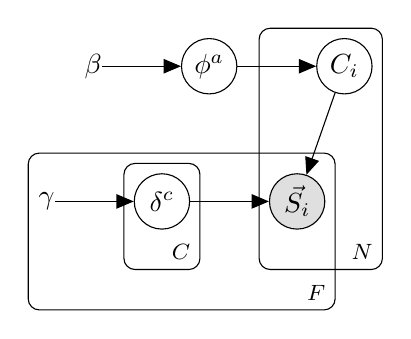
\begin{tikzpicture}
\node[latent] (c) {$C_{i}$};
\node[obs, below=of c, xshift=-0.6cm] (s) {$\vec{S_{i}}$};
\node[latent, left=of c] (phi) {$\phi^{a}$};
\node[const, left=of phi] (beta) {$\beta$};
\node[latent, left=of s] (delta) {$\delta^{c}$};
\node[const, left=of delta] (gamma) {$\gamma$};


\edge {phi}{c};
\edge {delta, c}{s};
\edge {beta}{phi};
\edge {gamma}{delta};


\plate {nutt}{(c)(s)}{$N$};
\plate {cvalue}{(delta)}{$C$};
\plate {fvalue}{(gamma)(delta)(s)(cvalue)}{$F$};
\end{tikzpicture}
\end{center}
\caption{Distributional learner}\label{fig:baseline-model}
\end{figure}

As we assume each morpho-syntactic feature follows the Bernoulli distribution, we can simplify our graph with a plate notation, with the plate $F$ representing the number of morpho-syntactic variables that the learner keeps track of (i.e. the variable $S$ repeats $F$ times). Each $S$ takes the value $1$ if the feature is present in the sentence, and $0$ otherwise. The probabilistic graphic model in Figure~\ref{fig:baseline-model} specifies the parameters and hyper-parameters of each variable with a plate notation. This learner assumes that each sentence is generated in the following way: the speaker chooses to use a certain clause type $C$, and then uses a set of morpho-syntactic features $\vec{S}$ (the number of features is $F$) to express this clause type. This process iterates $N$ times, $N$ being the number of sentences in the learner’s input. While the learner can observe the values assigned to $\vec{S}$ (represented by a shaded circle), they have to infer the value of $C$, namely their goal is to infer which clause type the speaker picked from the distribution of morpho-syntactic features of the sentence. Besides inferring the clause type of the current sentence, zooming out to the whole set of input sentences, the learner also tries to infer the probability distribution of all clause types in the input, as represented by the variable $\phi$ outside the plate $N$. Similarly, they also try to infer the probability distribution of the morpho-syntactic features ($\delta$) for each clause type across all input sentences. Namely, across all input sentences, for each clause type chosen by the speaker, how likely we would see a given feature present in the sentence. 

To put differently, the random variable $S$ is dependent on the random latent variable $C$. $C$ is in turn determined by the parameter $\phi$, which is determined by the hyperparameter $\beta$. In our model, $C$ follows multi-nominal distribution with three values, as corresponding to the three most prominent clause types (declarative, interrogative, imperative). $\vec{S}$ represents a set of morpho-syntactic features, each of which follows a Bernoulli distribution. The values for each morpho-syntactic features can be observed: if the feature is present in the current sentence, $S$ takes the value $1$, otherwise $0$. This variable is also controlled by a parameter $\delta$, indexed to $C$: each value of $C$ generates a different distribution of $\delta$ features occurring in a sentence is different depending on which clause type is being picked by the speaker. This parameter $\delta$ is controlled by a pre-determined hyper-parameter $\gamma$.


Here is a summary of the variables in the model, their meaning and distribution:

\begin{table}[H]
    \centering
    \begin{tabular}{c|l}
    \hline
    \hline
        C &  Clause Type, multinomial variable with 3 values\\
        & $ c \sim  \mbox{Multinomial}(\vec{\phi^{a}})$;\\
        &$\vec{\phi^{a}} \sim \mbox{Dir}(\beta)$\\
\hline
        $\vec{S}$ &  Morpho-syntactic features, feature bundle; \\
        & See Table~\ref{tab:eng-cl:formal-schema} for the full list of features included \\
        & $s^{(F)} \sim \mbox{Bernoulli}(\delta^{c})$ \\
        &$\delta\sim \mbox{Beta}(\gamma)$\\
    \hline
    \hline
    \end{tabular}
    \caption{Variables, their distribution, and explanation}
    \label{tab:baseline-variables}
\end{table}





\subsubsection{Inference}
\label{sec:engcl:model:baseline:infer}

The model infers the clause type category of each sentence through the method of Gibbs Sampling (\cite{geman1984gibbs}). I additionally assume the number of clause types is three. This assumption is based on the discussion that cross-linguistically, we see three major clause types: declaratives, interrogatives, and imperatives. It is therefore reasonable to start with a learner that tries to cluster the input sentences into three clusters. We will turn to the implication of this assumption, as well as propose a learner that does not adopt this assumption in Section~\ref{sec:engcl:disucssion}. 

The sampling process goes as follows. We first randomly initialize values of $C$ for each sentence with three categories (to represent declaratives, interrogatives, and imperatives). After initialization, I used the observed data in $\vec{S}$ for the current utterance and the values of $C$ of other sentences to calculate a posterior distribution over new category assignments for the current sentence, and then re-sample the new value of $C$ from this posterior probability distribution. This process was then repeated 5000 times, with the first 2500 iterations discarded as burn-in. Figure~\ref{fig:baseline-iter} shows the log of the joint probability of $C$ and $S$ at each iteration,  All parameters reached stable values within the burn-in period, and thus I will present values from the last iteration. The details of the sampling procedure and the pseudo-code of this Gibbs sampler can be found in Appendix~\ref{appx:eng-model-dir}; the code for this sampler can be found at \url{https://github.com/Yu-an/annotation_tool/blob/main/schema.pdf}. 

\begin{figure}[H]
    \centering
    \includegraphics[width=0.7\textwidth]{figures/baseline-iter.jpg}
    \caption{The log of the joint probability $p(C,\vec{S})$ at each iteration}
    \label{fig:baseline-iter}
\end{figure}


\subsubsection{Prediction} 
\label{sec:engcl:model:baseline:predict}
This learner simulates the learning process of infants, namely that the learning of clause type clustering happens in an unsupervised setting. We therefore predict that the model would not perform as well as a supervised learner who is given the true labels of clause type. 

Additionally, this learner serves as the baseline for our pragmatic syntactic bootstrapping learner, as it only learns the clustering of sentences from morpho-syntactic features. If this learner can achieve relatively good performance, our next question is then how much information from speech act (and socio-pragmatic information) contribute to the learning of clause types.


\subsubsection{Results}
\label{sec:engcl:model:baseline:results}

The data for this model were taken from the annotated dataset reported in the last section. The relevant features included in the model are: the presence/absence of subject, verb, verb morphology, auxiliary, subject-auxiliary inversion, sentence-initial unknown functional items, non-sentence-initial but pre-verbal unknown functional items, and post-verbal unknown functional items. We further filtered out sentences without verbs, as these fragments might not contain information about clauses, and it is possible that learners could make the distinction already at this age. The true labels of clause type were used to evaluate the performance of the model. As the learner needs to learn from sentences about clause-level properties, instead of one-noun utterances or utterances of only injectives, we eliminated from the dataset sentences that do not contain a verb or an auxiliary. In total, $3923$  sentences were fed into the model.


% \begin{figure}[H]
%     \centering
%     \includegraphics[width=0.5\textwidth]{figures/baseline-rand.jpg}
%     \caption{Performance of the model over 10 iterations measured by rand score}
%     \label{fig:baseline-rand}
% \end{figure}
Figure~\ref{fig:dist-compare-rand} shows the performance the distributional learner (10 rounds of simulation), in comparison to the supervised distributional learner. Rand score measures how similar the clustering result is to its gold-standard grouping; the closer the score is to 1, the better the performance. As expected, the distributional learner scores lower than the supervised learner. As will be seen, the main problem for the distributional learner comes from declaratives and imperatives, as a proportion of declaratives are clustered together with imperatives.

\begin{figure}[H]
    \centering
    \includegraphics[width=0.6\textwidth]{figures/dist-compare-rand.jpg}
    \caption{The performance of the distributional learner and the supervised distributional learner compared by rand score }
    \label{fig:dist-compare-rand}
\end{figure}


Figure~\ref{fig:baseline-heatmap} shows how much \diis{} in each cluster identified by the model. As can be seen, Cluster~$0$ contains 90\% of interrogative clauses and Cluster~$2$ is mostly declaratives. Cluster~$1$ is split between declaratives and imperatives.

\begin{figure}[H]
    \centering
    \includegraphics[width=0.7\textwidth]{figures/baseline-heatmap.jpg}
    \caption{The proportion of \diis{} in each of the three clusters}
    \label{fig:baseline-heatmap}
\end{figure}

Figure~\ref{fig:baseline-heatrev} shows the proportion of sentences clustered together. We can see that 87\% of interrogatives and 93\% of imperatives are clustered together in Cluster~$0$ and $1$ respectively. While most of declaratives are classified in Cluster~$2$, a proportion is classified in Cluster~$1$.

\begin{figure}[H]
    \centering
    \includegraphics[width=0.7\textwidth]{figures/baseline-heatrev.jpg}
    \caption{The proportion of actual \diis{} clustered in one category}
    \label{fig:baseline-heatrev}
\end{figure}

The distribution of formal features in each cluster is shown in Figure~\ref{fig:baseline-syncluster}, and three logistic regression models with each of the clusters as dependent variable, and the set of formal features (+/- verb and pre-verbal UFI are excluded, due to low variance) as independent variable are performed. Results of which is shown in Table~\ref{tab:baseline-synstats}.

\begin{figure}[H]
    \centering
    \includegraphics[width=1\textwidth]{figures/baseline-syncluster.jpg}
    \caption{The number of sentences with/without certain formal features in each cluster (Cluster 0 $\sim$ Interrogatives, Cluster 1 $\sim$ Imperatives, Cluster 2 $\sim$ Declaratives), darker colors represent the number of sentences with the feature. UFI stands for Unknown Functional Item (e.g. \twh{}), see Table~\ref{tab:eng-cl:formal-schema} for details.}
    \label{fig:baseline-syncluster}
\end{figure}

\begin{table}[H]
\begin{center}
\begin{tabular}{r|l|l|l}
\hline
 & Cluster~$0$   & Cluster~$1$   &  Cluster~$2$ \\
 & $\sim$ Interrogatives  & $\sim$ Imperatives  & $\sim$ Declaratives \\
 \hline\hline
constant & -6.97*** & 4.461*** & -4.22*** \\
\hline
Subject & 1.00* & -4.49*** & 4.37*** \\
\hline
Verb Morphology & -1.56*** & 0.21  & -1.46*** \\
\hline
Auxiliary & 3.4***  & -2.72*** & 1.16*** \\
\hline
Subject-Aux Inversion & 7.45*** & -5.83*** & -1.52*** \\
\hline
Sentence-initial UFI & 3.08*** & 0.38* & -1.58*** \\
\hline
Post-verbal UFI & -0.51  & -3.07***  & 1.69*** \\
\hline \hline
\end{tabular}
\end{center}
\caption{Results from the three logistic regression models with each of the clusters as the dependent variable and the morpho-syntactic features as independent variables; asterisks represent the significance level: ‘***’ 0.001 ‘**’ 0.01 ‘*’ 0.05 ‘.’ 0.1 ‘ ’ 1}
\label{tab:baseline-synstats}
\end{table}%


From the above table and figure, we can see that the model clearly identifies a cluster for interrogatives, and that features associated with polar and \twh-interrogatives are both present in this cluster. Interestingly, both subject and object \twh-interrogatives are included in this cluster:
\bex{engcl:baseline:cluster0}
Who's hiding in the barrel? \hfill Mother of Violet, Session 010603
\ex What else do we have here? \hfill Mother of Naima, Session 001126
\eex

Thee other two clusters are not as ideal. Cluster~$1$ consists of a mix of imperative sentences and simple declarative sentences like (\ref{engcl:baseline:cluster1-dec}):

\bex{engcl:baseline:cluster1-dec}
It's moon face. \hfill Mother of Lily, Session 010423
\ex I love school. \hfill Mother of Lily, Session 010423
\eex

Ambiguous sentences (sentences that could either be a pro-drop declarative or an left-edge-ellipsis interrogative) like \ref{engcl:baseline:cluster1-amb} are also put in Cluster~$1$:
\bex{engcl:baseline:cluster1-amb}
Wanna read your little Tigger book? \hfill Mother of Violet, Session 010407
\eex


Overall, the distributional learner fails to identify two of the three clause types in English, and fails to identify the characteristic features for imperatives and declaratives. We will turn to the pragmatic distributional learner next, to evaluate whether the learner needs information from pragmatics to identify clause types.

%As we have discussed, infants do not have access to the real labels of clause types. A more realistic model for infant language learning would be unsupervised model where they discover the clustering of sentences. In the next sections, we will compare two learners that have to learn clause type categories without access to the true labels, which mimics the learning process of language learning by infants: the distributional learner and the pragmatic distributional learner. 


\subsection{Pragmatic distributional learner}
\label{sec:engcl:model:pragmatics}

As we have discussed in Section~\ref{sec:engcl:background}, the learner needs to solve two problems: clustering the sentences, and labeling the clusters. We additionally see that speech act information is necessary to solving the labeling problem. The question then is, do learners need this information source to solve the clustering problem. As clause type categories are formal categories, theoretically we might not need information from the function of a sentence to identify these formal categories. However, as we have seen in the last section, a learner with only formal features cannot identify all three clause types. In this section, we will test the pragmatic distributional learner, to see if their performance improves.

Using speech act information also does not necessarily means that the performance of the learner improves, since speech acts could potentially be expressed by any type of clause type, and vice versa. It remains to be seen whether this source of information helps the learner or hurts the learner. 

We have seen in Section~\ref{sec:engcl:corpus:supervised}, in a supervised learning setting where the model is trained on actual clause type category data, adding pragmatics to the model improves model performance. But we also discussed that infants are not given the actual labels. In this section, we are building the pragmatic distributional learner with a Bayesian Clustering Model again, where the model infers clause type clustering without actual clause type labels. 

In this section, I will first detail the specification of the pragmatic distributional learner, which is given speech act information and information about morpho-syntactic features, to infer clause typing. I then compare the performance of the two learners (and their supervised counter-parts). As we will see, the pragmatic distributional learner outperforms the distributional learner. Speech act also provides a much higher performance boost for our unsupervised learners, as the improvement is much higher than their supervised counterparts.


\subsubsection{Model Specification}
\label{sec:engcl:model:prag:spec}


Similar to the distributional learner, the pragmatic distributional learner is also a Bayesian Clustering Model. The learner is given speech act information ($A$) in addition to the morpho-syntactic features ($\vec{S}$). The pragmatic distributional learner assumes that each sentence is generated in the following way: the speaker of the sentence first chooses a particular speech act ($A$), then picks one out of three clause types to express the speech act, and finally picks what kind of formal figures to use. 



\begin{figure}[H]
\begin{center}
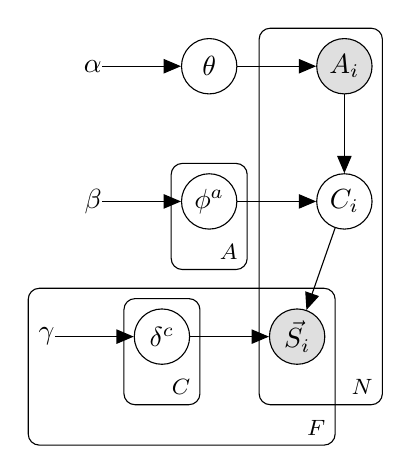
\begin{tikzpicture}
\node[obs] (a) {$A_{i}$};
\node[latent, left=of a] (theta) {$\theta$};
\node[const, left=of theta] (alpha) {$\alpha$};
\node[latent, below=of a] (c) {$C_{i}$};
\node[obs, below=of c, xshift=-0.6cm] (s) {$\vec{S_{i}}$};
\node[latent, left=of c] (phi) {$\phi^{a}$};
\node[const, left=of phi] (beta) {$\beta$};
\node[latent, left=of s] (delta) {$\delta^{c}$};
\node[const, left=of delta] (gamma) {$\gamma$};

\edge {theta}{a};
\edge {alpha}{theta};
\edge {phi, a}{c};
\edge {delta, c}{s};
\edge {beta}{phi};
\edge {gamma}{delta};


\plate {nutt}{(a)(c)(s)}{$N$};
\plate {avalue}{(phi)}{$A$};
\plate {cvalue}{(delta)}{$C$};
\plate {fvalue}{(gamma)(delta)(s)(cvalue)}{$F$};
\end{tikzpicture}
\end{center}
\caption{Pragmatic distributional learner}\label{fig:target-model}
\end{figure}

Figure~\ref{fig:target-model} shows the graphical model of the learner. The model assumes that the latent variable $C$ depends on the value of an observed variable $A$. This variable $A$ follows a multi-nominal distribution with parameter $\theta$, representing the probability distribution of each speech act in the input. The parameter for $C$ is still $\phi$, but this time $\phi$ is indexed to values of $A$, namely for each speech act, the distribution over different clause types might be different. Similar to the distributional learner, morpho-syntactic features are again represented by $\vec{S}$, which contains a set of formal features (the same ones as in the distributional learner). $\vec{S}$ is dependent on $C$ and the parameter $\delta$. 

This learner's task is to infer the category $C$ of each sentence with the observed surface formal features, as well as the speech act information. In this section, we assume that the learner has access to the speech act information. Here our goal is to simply test the idea that if the learner is given data about the function of a clause, will its performance in solving the clustering problem improve.

In the next section, we will examine how much information from speech act the learner actually needs by manipulating the amount of noise in speech act information. One might wonder how children might bootstrap into the different speech act categories in the first place. We will turn to some possible sources for speech act categorization in Chapter~\ref{chap:eng-sp}.

Besides trying to infer the value of $C$ for each utterance, the learner also needs to learn the probability distribution of each clause type associated with each speech act. Note that this is a rather simplified representation of the relation between clause type and speech act, further research is needed to model the relationship between form and function (see \cite{gong2021rsaq} for an attempt to use rational speech act theory to capture this form-function relation).



Here is a summary of the variables in the model, their meaning and distribution:

\begin{table}[H]
    \centering
    \begin{tabular}{c|l}
    \hline
    \hline
    
        A & Speech Act, four values: Assertion, Question, Request/Command, other\\
        & $ a \sim \mbox{Multinomial}(\vec{\theta})$;\\
        & $\vec{\theta} \sim \mbox{Dir}(\alpha)$\\
\hline
        C &  Clause Type, multinomial variable with 3 values\\
        & $ c \sim  \mbox{Multinomial}(\vec{\phi^{a}})$;\\
        &$\vec{\phi^{a}} \sim \mbox{Dir}(\beta)$\\
\hline
        $\vec{S}$ &  Syntactic features, feature bundle; \\
        & the value of each feature $F$ is $S^{(F)}$ \\
        & $s^{(F)} \sim \mbox{Bernoulli}(\delta^{c})$ \\
        &$\delta\sim \mbox{Beta}(\gamma)$\\
    \hline
    \hline
    \end{tabular}
    \caption{Variables in the pragmatic distributional learner, their distributions, and explanations}
    \label{tab:target-variables}
\end{table}


\subsubsection{Inference}
\label{sec:engcl:model:prag:infer}




The sampling process is similar to that in the last section. We first randomly initialize values of $C$ for each sentence with three categories (to represent declaratives, interrogatives, and imperatives). After initialization, I use the observed data in $A$ and the observed data in $\vec{S}$ for the current utterance and the values of $C$ of other sentences to calculate a posterior distribution over new category assignments for the current sentence, and then re-sample the new value of $C$ from this posterior probability distribution. Again, a Gibbs sampler similar to that for the baseline model was implemented, and the sampling procedure repeated for 5000 times with the first 2500 discarded as burn-in. Values of all parameters converged to a stable state within the burn-in period, and therefore the values from the last iteration will be reported here.  Figure~\ref{fig:baseline-iter} shows the log of the joint probability of $C$ and $S$ at each iteration.  All parameters reached stable values within the burn-in period, and thus I will present values from the last iteration. %The details of the sampling procedure and the pseudo-code of this Gibbs sampler can be found in Appendix~\ref{appx:eng-model-dir}; the code for this sampler can be found URL. 

\begin{figure}[H]
    \centering
    \includegraphics[width=0.7\textwidth]{figures/target-iters.jpg}
    \caption{The log of the joint probability p(A,C,$\vec{S}$) across 5000 iterations}
    \label{fig:target-iters}
\end{figure}




\subsubsection{Prediction}
\label{sec:engcl:model:prag:predict}


If learners do need function information to cluster sentences, we will see the pragmatic distributional learner outperforms the distributional learner. However, this learner is still an unsupervised learner, in that it is not trained on the actual clause type labels in the corpus, so its performance might be lower than the supervised models.



\subsubsection{Results}
\label{sec:engcl:model:prag:results}

We draw the data for simulation from the same dataset, this time with speech act information. Overall, the model outperforms the distributional learner. As can be seen from Figure~\ref{fig:compare-rand}, the rand score (which measures how well two clusters coincide with each other) of the pragmatic distributional learner is higher. Additionally, the difference between the pragmatic and the distributional learner is larger than the difference between the two supervised learners, suggesting that for learners without access to the actual labels of clause types (which we assume to be the best approximation to the language acquisition process of infants), speech act information is crucial not only for labeling, but also clustering. 


\begin{figure}[H]
    \centering
    \includegraphics[width=0.6\textwidth]{figures/compare-rand.jpg}
    \caption{Comparing all four learners (distributional, pragmatic distributional, supervised distributional, supervised pragmatic) by rand score }
    \label{fig:compare-rand}
\end{figure}




Figure~\ref{fig:target-heatmap} shows how much \diis{} in each cluster identified by the model. As can be seen, the model is able to identify three clause clusters: Cluster~$0$ contains 94\% of interrogative clauses, Cluster~$2$ is mostly imperatives, and Cluster $1$ mostly declaratives. 

\begin{figure}[H]
    \centering
    \includegraphics[width=0.7\textwidth]{figures/target-heatmap.jpg}
    \caption{The proportion of \diis{} in each of the three clusters}
    \label{fig:target-heatmap}
\end{figure}

Figure~\ref{fig:target-heatrev} shows the proportion of sentences clustered together. We can see that our learner performs extremely well: 95\% of declaratives, 90\% of interrogatives, and 87\% of imperatives are clustered together in Cluster~$1$, $0$, $2$ respectively.


\begin{figure}[H]
    \centering
    \includegraphics[width=0.7\textwidth]{figures/target-heatrev.jpg}
    \caption{The proportion of actual \diis{} clustered in one category}
    \label{fig:target-heatrev}
\end{figure}


Figure~\ref{fig:target-syncluster} shows the presence of morpho-syntactic features in each cluster; Table~\ref{tab:target-synstats} summarises the three logistic regression models with each of the clusters as dependent variable, and the set of formal features (+/- verb and pre-verbal UFI are excluded, due to low variance) as independent variables.  

\begin{figure}[H]
    \centering
    \includegraphics[width=1\textwidth]{figures/target-syncluster.jpg}
    \caption{The number of sentences with/without certain formal features in each cluster (Cluster 0 $\sim$ Interrogatives, Cluster 1 $\sim$ Declaratives, Cluster 2 $\sim$ Imperatives), darker colors represent the number of sentences with the feature.}
    \label{fig:target-syncluster}
\end{figure}


\begin{table}[H]
\begin{center}
\begin{tabular}{r|l|l|l}
\hline
 & Cluster~$0$   & Cluster~$1$   &  Cluster~$2$ \\
 & $\sim$ Interrogatives  & $\sim$Declaratives  & $\sim$ Imperatives \\
 \hline\hline
constant & -6.3*** & -1.44*** & 1.95*** \\
\hline
Subject & 0.9** & 4.32*** & -4.75*** \\
\hline
Verb Morphology & -0.31 & 1.66***  & -3.08*** \\
\hline
Auxiliary & 2.66***  & -0.85*** & -2.14*** \\
\hline
Subject-Aux Inversion &5.99*** & -5.83*** & -56.79 \\
\hline
Sentence-initial UFI & 3.65*** & 0.38* & 0.72** \\
\hline
Post-verbal UFI & -0.43  & 0.5  & -1.12 \\
\hline \hline
\end{tabular}
\end{center}
\caption{Results from the three logistic regression models with each of the clusters as the dependent variable and the morpho-syntactic features as independent variables; asterisks represent the significance level: ‘***’ 0.001 ‘**’ 0.01 ‘*’ 0.05 ‘.’ 0.1 ‘ ’ 1}
\label{tab:target-synstats}
\end{table}%

% \begin{figure}[H]
%     \centering
%     \includegraphics[width=0.6\textwidth]{figures/target-base-rand.jpg}
%     \caption{Comparing the pragmatic distributional learner and the distributional learner by rand score }
%     \label{fig:target-base-rand}
% \end{figure}


The distribution of formal features across the three clusters is similar to the distribution with actual clause type categories. Cluster $0$, the interrogative cluster, is associated with the presence of subject-auxiliary inversion and sentence-initial unknown functional items (UFIs); Cluster $2$, the imperative cluster, is associated with the absence of subject, auxiliaries, verb morphology, or UFIs. The declarative cluster Cluster $1$ is correlated with the presence of subjects, verb morphology, and the lack of subject-auxiliary inversion. The three clusters match the actual clause types, \diis.

Comparing the pragmatic distributional learner with the distributional learner, we can see that the former performs much better, identifying all three clause types and the prominent features associated with these clusters. These results suggest the learner needs information from pragmatics to succeed in clause typing. But how much does the learner need pragmatics? Will noisy speech act information still able to help the learner? In the next section, we compare pragmatic distributional learners with different levels of noises in their speech act information, and see how well the learner performs with deprecated data.

\subsection{Noisy pragmatic distributional learner}
\label{sec:engcl:model:noisy}

\subsubsection{Simulating noisy A}
The model is the same as the pragmatic distributional learner discussed in the last section, but instead of taking true speech act labels as input, the model was fed noisy speech act information. With this manipulation, we would be able to see how much the model can handle noise from speech act information. 




\begin{figure}[H]
\begin{center}
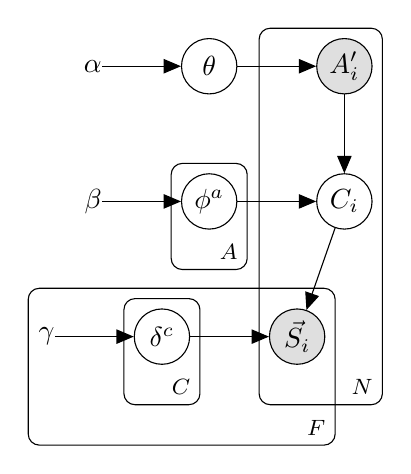
\begin{tikzpicture}
\node[obs] (a) {$A'_{i}$};
\node[latent, left=of a] (theta) {$\theta$};
\node[const, left=of theta] (alpha) {$\alpha$};
\node[latent, below=of a] (c) {$C_{i}$};
\node[obs, below=of c, xshift=-0.6cm] (s) {$\vec{S_{i}}$};
\node[latent, left=of c] (phi) {$\phi^{a}$};
\node[const, left=of phi] (beta) {$\beta$};
\node[latent, left=of s] (delta) {$\delta^{c}$};
\node[const, left=of delta] (gamma) {$\gamma$};

\edge {theta}{a};
\edge {alpha}{theta};
\edge {phi, a}{c};
\edge {delta, c}{s};
\edge {beta}{phi};
\edge {gamma}{delta};


\plate {nutt}{(a)(c)(s)}{$N$};
\plate {avalue}{(phi)}{$A$};
\plate {cvalue}{(delta)}{$C$};
\plate {fvalue}{(gamma)(delta)(s)(cvalue)}{$F$};
\end{tikzpicture}
\end{center}
\caption{Pragmatic distributional learner}\label{fig: noisy-model}
\end{figure}

In this model, we replace the true labels of the speech act variable $A'$ with a noisy version of $A$. A portion of the observations of $A'$ will be replaced by noise. To make the simulation, I replace 0 to 100\% of the true labels of speech act information with random labels. The goal of the model is to see at what noise level would the speech act information affects the inference of clause type categories. 

I again adopt the Gibbs sampling method to infer the parameter values, same as for the last two models. The sampling procedure repeat 5000 times with the first 2500 discarded as burn-in. Values of all parameters converge to a stable state within the burn-in period, and therefore the values from the last iteration will be reported here. 

\subsubsection{Results}
\label{sec:engcl:model:noisy:results}

Figure~\ref{fig:noisy-rand-compare} shows the performance of the pragmatic distributional learner when the speech act contains 0-100\% noise. As can be seen, the learner outperforms the distributional learner up until there is around 85\% of noise in speech act. This suggests that speech act information is helpful for learners to cluster sentences, and even deprecated speech act information will still help the learner.  

\begin{figure}[H]
    \centering
    \includegraphics[width=1\textwidth]{figures/noisy-rand-compare.jpg}
    \caption{Compare the performance of pragmatic distributional learners taking different levels of noisy speech act information; dotted marks the rand score of the distributional learner}
    \label{fig:noisy-rand-compare}
\end{figure}

Looking at the learner at maximum noise level, we can see that the model fails to identify a cluster for declaratives (Figutre~\ref{fig:noisy100-heatmap}. Similar to the distributional learner, the cluster for imperatives also have declaratives (\ref{fig:noisy100-heatrev}). 



\begin{figure}[H]
    \centering
    \includegraphics[width=0.7\textwidth]{figures/noisy100-heatmap.jpg}
    \caption{The proportion of \diis{} in each of the three clusters (100\% noise in speech act information) }
    \label{fig:noisy100-heatmap}
\end{figure}

\begin{figure}[H]
    \centering
    \includegraphics[width=0.7\textwidth]{figures/noisy100-heatrev.jpg}
    \caption{The proportion of actual \diis{} clustered in one category}
    \label{fig:noisy100-heatrev}
\end{figure}

Looking at the distribution of syntactic features, we can see that the model has the same problem as the distributional learner. Cluster $0$, which should be the imperative cluster, still have sentences that have subjects. 

\begin{figure}[H]
    \centering
    \includegraphics[width=1\textwidth]{figures/noisy100-syncluster.jpg}
    \caption{The number of sentences with/without certain formal features in each cluster (Cluster 0 $\sim$ Interrogatives, Cluster 1 $\sim$ Imperatives, Cluster 2 $\sim$ Declaratives), darker colors represent the number of sentences with the feature.}
    \label{fig:noisy100-syncluster}
\end{figure}




\subsection{Interim Discussion}
\label{sec:engcl:model:disc}
In summary, the speech act information is very tolerant of noises. The pragmatic distribution learner consistently outperforms the distributional learner, and only drops when the noise in speech act reaches 85\%. 

These results suggest that pragmatic information is crucial to the learner, not just to solve the labeling problem, but also to help with clustering. 

\section{Discussion}
\label{sec:engcl:discussion}

In this chapter, we looked at how learners might learn to categorize sentences. We first examined the patterns in parents' input, and see that parents use clause types systematically, and that the three clause types are predominantly mapped to their canonical functions (declaratives to assertions, interrogatives to questions, imperatives to requests/commands). The three clause types are also used systematically, with their formal features consistently present in the input sentences. 

We then address the question of how infants might succeed at the clustering task. Specifically, do they need pragmatic information to solve the clustering problem? Given the fact that clause types are formal categories, it is at first glance reasonable to assume that infants are able to identify the main clause types with formal features only. We build two learners, the distributional learner and the pragmatic distributional learners to probe this question. The distributional learner learns clause typing from formal features only, but the pragmatic distributional learner also has access to the speech act information. We find that the pragmatic distributional learner outperforms the distributional learner, suggesting that pragmatic information is necessary, even for clustering. We then manipulated the level of noise in speech act, to see how tolerant this information source can be. Turns out, even if the pragmatic distributional learner is given speech act information with 85\% of noise, they still outperforms the distributional learner. 

From these results, we conclude that pragmatics is essential for learning clause typing. Infants learn how to cluster sentences into clause types by observing the formal features of the sentences, together with speech act information.

Our next question is then, what about other languages? As we have discussed in Chapter~\ref{chap:litreview}, languages differ in the formal features of each clause type, and learners need to discover the correlation from input. The distributional learner for English still have some success with clustering, identifying interrogative clauses. However, maybe the formal features are not as informative in other languages. In the next chapter, we will turn to Mandarin learners, and test the two learners with Mandarin input data. 

Another question remains is that, how does the pragmatic distributional learner identify speech act information? While it is indisputable that information from clause type should be necessary, are there any non-clause type information about speech act in their everyday interaction with parents? In Chapter~\ref{chap:eng-sp}, we will turn to the learning of speech acts from non-clause type information.





\chapter{Learning to identify clause types in Mandarin}
\label{chap:man-cl}

\section{Background}
\subsection{Clause types in Mandarin}

\subsection{Mandarin-acquiring children's knowledge of clause types}

\subsection{Roadmap of the chapter}

\section{Corpus study}

\section{Models}
\subsection{The \distlearner{}}
\subsection{The \praglearner{}}
\subsection{Manipulating ratio of noise in pragmatic information}

\section{Discussion}






\chapter{Learning speech acts}
\label{chap:eng-sp}

As we have discussed in the last three chapters, pragmatics is crucial for children to learn clause type categories, and even noisy pragmatics can benefit the learner. But then, there still remains the question of how children learn speech act categories? Given that the way we generally identify a speech act is via its clause type, there is a potentially vicious circle here: you need to know the clause type to identify the speech act, but you need to know the speech act to identify the clause type. %How do learners avoid this circularity? 

But as we have discussed in Chapter~\ref{chap:introduction}, it is likely that children learn to identify speech act and clause type in tandem and mutually informative ways: children learn to identify clause types by tracking morpho-syntactic and prosodic regularities in conjunction with their growing
knowledge of speech act and its associated behavioral cues; similarly, they learn
to identify speech acts by tracking social pragmatic cues and prosodic cues in conjunction with their growing
understanding of the formal features of various clause types.


In Chapter~\ref{chap:eng-cl} and~\ref{chap:man-cl}, we have seen that even if children have limited access to the speech act information, they might still benefit from it when learning to cluster clause types. If children do not need \emph{perfect} speech act information to figure out clause types, then we do not need to assume that by the time children are learning to figure out clause types, they have already figured out speech acts. 

But what about the learning of speech act categories? Even if children must rely on clause type information to figure out speech acts, they could have access to additional information that is unrelated to clause typing, but informative for recognizing speech act type. For example, in conversations, we use questions to elicit responses and information, which leads to behaviors like pausing after questions, or looking directly at our interlocutor, to nudge them to answer our questions. Thus, armed with an innate category for questions, and a theory of what questions do in conversations, the child can expect certain kinds of nonlinguistic behavior to be correlated with the act of asking a question. If these behaviors are also correlated with the act of asking a question in the input, then they can tell whether their parent is asking them a question.  

But just as surface formal features might be absent or misleading in the input, the social pragmatic features might also be absent or misleading. Therefore, I ask in this chapter whether it is possible to see some social pragmatic and prosodic features correlated with speech acts. I focus on the questioning act here, as this speech act is relatively well understood, and plan to extend to requests/commands in the future.

In conversations, questions are devices for us to engage with an addressee. When we ask questions, we are looking for information, or sometimes simply for a response. This makes questions perfect turn-transition points (\cite{duncan1972turn} among many others), signaling that the current speaker is done with the turn and the next speaker needs to get ready. This makes the use of questions to be correlated with  communicative signals like direct eye gaze: speakers gaze at their interlocutor longer after questions (\cite{argyle1972gaze}). When we are looking at our interlocutor for an answer, we might have certain facial expressions. For example, \textcite{domaneschi2017facial} find people tend to associated with the facial expressions pictured in Figure~\ref{fig:engsp:au} with questions. If children are equipped with the knowledge about facial expressions, they might be able to exploit the correlation between questioning and facial expressions to learn about questions. 
\begin{figure}[H]
    \centering
    \includegraphics[width=1\textwidth]{figures/q-aus.jpg}     
    \caption{The upper face action units (AU) identified by participants as indicating the act of questioning, as reported by \cite{domaneschi2017facial}}
    \label{fig:engsp:au}
\end{figure}

Another similar conversational signal might be the time in-between conversational turns. A property related to a turn-transition point is that interlocutors use these points as cues for when to take over the turn. In a natural face-to-face conversation, the gap between a question and its answer might be smaller than other pairs of utterances in a conversation (\citealt{tice2011turn} a.o.). But the questioner might also pause and wait if nobody steps in immediately (\cite{sacks1978pause}). Therefore, tracking the gap after utterances might tell us whether the utterance is a question.


So if children understand the mechanism of human communication, which as we have in Chapter~\ref{chap:background} that they do, and have the prior knowledge that certain speech acts expects responses, they might expect to see a correlation between questions and the length of eye gaze, the facial expressions of their interlocutor, and the length of pauses. They then can exploit this correlation to learn questions.

We express our desire to know with questions (e.g.\cite{searle1975tax, krifka2011q, carruthers2018q}). As a result, when we ask questions, we might be ignorant of certain information. If children can keep track of who knows what, and as we saw in Chapter~\ref{chap:background} that they can, they can exploit this correlation between lack of information with questions to infer questionhood. However, this correlation might not show up in the input, as parents tend to use questions as a tool for teaching. A parent asking ``What's that?'' is likely not to solicit some information they don't know, but to see if the child knows it too. Previous corpus study suggests that about 38\% of parents' questions when the child is before 2 years old are pedagogical questions (\cite{yu2019pedagogical}), and for middle class parents, this number could reach 60\%. The child might still be able to exploit the cue in some way, but it might not be as straightforward.  

Due to the limitation of our corpus data, in this chapter we will examine the following features: duration of pauses between utterances and eye gaze. This chapter is organized as follows: Section~\ref{sec:engsp:background} reviews previous evidence for children's perception of these cues. I then report results from a corpus study with Providence Corpus in Section~\ref{sec:engsp:corpus}, where I looked at the length of pauses between parents' utterances (Section~\ref{sec:engsp:results:pause}) and parents' attentional behavior (\ref{sec:engsp:results:gaze}).
Section~\ref{sec:engsp:discussion} concludes the chapter.


\section{Background}
\label{sec:engsp:background}
\subsection{Pauses in conversation}
\label{sec:engsp:bg:pause}
As mentioned earlier, questions are turn-transition points (\cite{duncan1972turn} among others), and this means that speakers anticipate a change of turn after questions. In adult-to-adult conversations, this property translates to shorter speech gaps after questions in one-on-one in-person conversations (\cite{stivers2010,enfield2010,hilbrink2013turn} among many others). Speakers might also wait after questions for responses (\cite{sacks1978pause}), but for adults, longer inter-turn silence leads to feelings of unease and tend to be avoided (\cite{roberts2006pause} among others). But when interacting with pre-linguistic infants, this silence might be helpful rather than awkward: if children can track the length of pause after an utterance, they might be able to infer that longer pauses are associated with questions and request. Are children sensitive to the turn-taking properties of conversations? 
%As infants could use prosodic cues to detect clause boundaries (\cite{hirsh1987clause, seidl2007prosody}), they might be able to track the length of pause after an utterance. 

As early as 3 months old, infants show sensitivity to the structure of conversation. The overlap between infant vocalization and parents' speech decreases overtime, and the average gap between parent utterance and infant vocalization decreases, suggesting that they respect the turn-taking rules (\cite{hilbrink2013turn3mo}). When they start producing one-word utterances, slow down at trying to change turn, but quickly pick up the speed again as their linguistic ability develops (\cite{hilbrink2013turn}).

Studies also show that same as adults, children interpret pauses as meaningful. \textcite{craiggallagher1983pause} 
investigate whether or not 22-36-month-olds abandon their request (e.g. wanting a cookie) after the parent's initial responses (classified as neutral, e.g. \tit{you want what?},  negative, \tit{No.} or pause). They found that the older children (3-year-olds) abandon requests after adult pauses for more than 1s, suggesting that children treat long pauses as a meaningful response. This is suggestive, but based on this research alone it remains unclear whether children associate inter-turn silence with the interlocutor trying to elicit a response. 

%Bloom et al: four children, 21 to 36 months of age. Adjacent speech is more than anything from the beginning, Contingent speech increase over time (adjacent (immediately preceded by an adult utterance), or as nonadjacent (not immediately preceded by an adult utterance). Adjacent utterances were either contingent (shared the same topic and added new information relative to the topic of the prior utterance), imitative (shared the same topic but did not add new information), or noncontingent (did not share the same topic). Linguistically contingent speech (speech that expanded the verb relation of the prior adult utterance with added or replaced constituents within a clause)  occurred more often after questions than nonquestions. 

On the other side the problem, the length of pauses results from the dynamics of conversation; if parents are interacting with a pre-linguistic infant, would they follow the same rules? In other words, if we assume that children can keep track of the length of pauses, are there any patterns found in the silences? Previous studies show that parents seem to treat even pre-linguistic infants as competent conversationalists, and any vocalizations (e.g. crying, babbling) or even body movements, are treated as a conversational turn (\cite{beebe1988,jaffe2001turn}). The length of pauses also correlates with the vocabulary of children (\cite{marklund2015pause}). Different from adult-to-adult interactions, parents of 14-month-olds tend to follow questions with another question (\cite{reimchen2017}).  

While these studies show that parents respect turn-taking rules when interacting with pre-verbal infants, little is known about whether parents' speech gaps are informative of the speech act performed. To address this problem, Section~\ref{sec:engsp:results:pause} examines the correlation between the speech act of an utterance and the length of pauses after an utterance, to see if the gap between utterances is informative of an utterance's speech acts. 

\subsection{Attentional behavior}
\label{sec:engsp:bg:gaze}

Another consequence of the response-expectation property of questions is that by the end of a question, the speaker tends to appoint the next speaker. A common device for turn allocation is eye gaze (\citealt{argyle1972gaze, kendon1967gaze,duncan1979gaze, rossano2009gaze, csibra2010}). In dyadic interactions, we tend to look at our interlocutor when we need their response. Thus, it is possible that by tracking where the parent attends to, specifically whether the parent is directly looking at the learner, the learner might be able to infer whether a question is being asked. 

We have seen in Chapter~\ref{sec:bg:acq:pre} that infants are sensitive to the direction of eye gaze since birth. 3-day-old newborns prefer to look at the face that appears to make eye contact with them, suggesting that they are sensitive to the position of the pupils/irises within the eye (\cite{farroni2004gaze}).


While these studies show that infants can perceive parents' direction of eye gaze, and that adults use eye gaze for turn allocation, so far little is known about whether parents' gaze pattern correlates with turn allocation, and furthermore, with the speech act of an utterance. If questions signals a transition of turn, parents' gaze should fall on the addressee--the child--more after questions. I address this question in Section~\ref{sec:engsp:results:pause} by examining parents gaze pattern during parent-child interactions, to see if this cue is informative of an utterance's speech acts.

\subsection{Interim Summary}
\label{sec:engsp:bg:summary}

When interacting with other people, we use many cues, besides the clause type information, to infer what kind of speech act is being performed. In particular, since questions usually signal the transition of a conversational turn, the questioner usually shifts gaze to the next designated speaker. Adults can also infer from a question being performed that the questioner wants someone to pick up the turn, and thus the lengths of speech gap after questions are normally longer than lengths of pause after other speech acts. However, if we look at dyadic interactions between a parent and a child, especially a child as young as 18 months old, these cues might not show up, or show up in a different way. We should ask, for example, whether parents in child-directed interaction also use direct eye gaze to indicate the next speaker, i.e. the child? Also, since 18-month-olds are not mature conversationalists, the speech gap after utterances might be longer across the board, so are there any differences in pauses that correlate with the speech act being performed? Another potential cue is prosody. In English, yes/no questions are usually associated with a special final rise contour (L* H-H\%), which can be produced with either polar interrogatives and declaratives syntax. Would final rises be a cue that distinguishes between the three speech acts?

To address these questions, we built a multi-modal dataset with dyadic parent-child interactions for infants before 18 months old, to see if there is any non-clause type cues that may help infants distinguish speech acts.

\section{Corpus study}
\label{sec:engsp:corpus}

This section details the corpus study we conducted to investigate whether speech gap, direct gaze, and prosody in dyadic parent-child interactions correlate with parents' use of different speech acts. 


\subsection{Methods}
\label{sec:engsp:corpus:method}
This study also used data from the Providence Corpus (\citealt{ProvidenceCorpus}) from CHILDES system (\citealt{CHILDES}). The audio and video of the sessions sampled in Chapter~\ref{chap:eng-cl} and Chapter~\ref{chap:prosody} were extracted for annotation. 


For annotating gaze, we used the video data available in the Providence corpus. Trained annotators viewed the muted videos using ELAN (\cite{elan}). Each video was annotated first with whether the parent and the child are visible on screen and the parent's focus of attention can be identified. If the parent is only half on screen, but we can still identify the focus of attention of the parent, this proportion was counted as on-screen. If the parent is on screen but the focus cannot be identified due to bad lighting, this proportion of the video was counted as off-screen.

Then, for the parts of the video that both the parent and the child are both on screen, the focus of parents' attention was annotated. Specifically, whether the parent is paying attention to the child, to an object, or unidentifiable. The parent was annotated as paying attention to the child when they attended to the child through (1) direct eye gaze (when the eyes could be seen), (2) head or body orientation toward the child (when the eyes could not be seen), (3) physical interaction with the child. I then used a script to calculate the proportion of looks to the child during the utterance, and at 1s, 2s, 3s before and after the utterance.%, by dividing the total length of the on-screen time by the length that the parent attends to the child.  
 
\subsection{The correlations we expect}
\label{sec:engsp:predictions}
If speech gaps and gaze are indeed useful cues to obtain speech act information, we would expect the following predictions to bear out.


For speech gaps, we should see that parents pause longer after questions and requests than after assertions, to wait for responses.
And for eye gaze, we should see that parents direct attention to the child more often after questions and requests than after assertions. 


\subsection{Results}
\label{sec:engsp:results}

\subsubsection{Pauses}
\label{sec:engsp:results:pause}

For this cue, we measured the length of silence between parents’ consecutive utterances like (\ref{code-prag:pause}). To do so, we first followed the methodology of \textcite{bloom1976discourse} and annotated for each utterance whether it is a contingent utterance of the previous one, i.e.\ whether it shares the same topic and adds new information relative to the topic of the prior utterance. We will refer to such pairs of utterances, with one contingent on the previous utterance like in (\ref{code-prag:pause}), as consecutive turn sequences. Within the sequences, I measured the length of pauses between utterances. 


\bex{code-prag:pause}
%\bxl{}
\tbf{Consecutive turn sequence}
\bxl
You can’t take your rake on the swing.\\
 \tsc{pause: 0.014s} \\ 
 You wanna take your big bird rake on the swing? 			\hfill \tsc{Assertion -Question}
\ex You don't wanna swing?\\
 \tsc{pause: pause: 0.23s} \\	
 You don’t have to.	\hfill \tsc{Question-Assertion}
\ex Here you use this one. \\
 \tsc{pause:  0.033s} \\ This one works better.	\hfill \tsc{Assertion-Assertion}
\exl
\eex

In total, 4066 utterances were found to have a contingent follow-up that allows us to measure the inter-turn silence. Figure~\ref{fig:engsp:pause} shows the length of pause after each speech act category.

\begin{figure}[H]
\begin{center}
\includegraphics[width = 0.8\textwidth]{figures/pause.jpg}
	\caption{Duration of pause (ms) after each type of speech act}\label{fig:engsp:pause}
\end{center}
\end{figure}

These results show that parents are equally likely to ask another question as they are to answer their own questions, but parents tend to pause longer after questions (mean $= 1728ms$) than assertions (mean $= 1321ms; t(2925) = -2.23, p = 0.02$), suggesting that parents pause after asking a question but proceed with the conversation after an assertion. %There is no difference between questions and requests mean $= 1345ms; t(1418) = 0.83, p = 0.4$), suggesting

\begin{comment}
\begin{figure}[H]
\begin{center}
\includegraphics[width = 0.8\textwidth]{figures/pause-QA.jpg}
	\caption{Duration of pause (ms) between Question-Question/Assertion and Assertion-Question/Assertion pairs }\label{fig:engsp:pause-QA}
\end{center}
\end{figure}
\end{comment}


\subsubsection{Parents' attentional behavior}
\label{sec:engsp:results:gaze}

In total, 857 utterances were found to have attentional data suitable for annotation. Figure~\ref{fig:attention} shows the proportion of looks to the child before, during, and after an utterance.


\begin{figure}[H]

\begin{center}
	\includegraphics[width =1\textwidth]{figures/gaze-pattern-adult.jpg}
	\caption{Proportion of parents' looks to the child before, during, and after an utterance} \label{fig:attention}
\end{center}
\end{figure}


From Fig.~\ref{fig:attention}, we can see that when the utterance is a question, the proportion of looks to the child is higher (average $0.41$) than when it is an assertion (average $0.27; t(16) = 2.53, p <0.05$), but roughly equivalent to when the utterance is a request ($0.37; t(16)= 1.27, p=0.21$). These results suggest that parents look at the child longer after questions and requests. %%%%; in the post-utterance region, the proportion of looks to the child is higher when the utterance is a question ($0.53$) than when it is an assertion ($0.25; t(4) = 7.95, p<0.05$) but not when it's a request ($0.39; t(4) = 4.2, p=0.2$). 

\begin{comment}


\subsubsection{Informativeness of the cues}
\label{sec:engsp:results:stats}
A multinomial logistic regression model was built with the three cues as independent variables, and the speech act categories (assertions, questions, requests, and other) as the dependent variable. The data for the model was an intersection of the prosody, pause, and attentional data, as not all utterances have follow-up utterances for us to measure the inter-turn silence, and some utterances were uttered off screen with no attentional data. In total, 806 utterances were included in the analysis.  We then split the data into a training set (90\% of the data) and testing set (10\%), and trained a logistic regression classifier with the training data. For details of the model, see Appendix~\ref{appx}. This classifier can predict 57\% of the speech act labels, suggesting that the three cues could to some extend help children identify speech act information. 
\end{comment}

\section{Conclusion}
\label{sec:engsp:discussion}
This chapter investigated the question of how children might be able to pick out speech acts independently of clause types or prosodic information. As questions are often used to elicit responses and information, we can expect different kinds of behavior to be correlated with these acts. Armed with an innate category for questions, and a theory of what questions do in conversations, the child can expect certain kinds of non-clause type cues to be correlated with the act of asking a question. 

Some candidates for cues that could potentially differentiate questions from other speech acts are pauses and direct eye gaze. The canonical function of questions is to solicit responses or seek information, so when we use questions, it is likely that we pause after questions, or look directly at our interlocutor, as a way to signal to them that they need to take over the conversational turn. As we have reviewed, children have a theory of communication early on, and understand the structure of conversations from as young as three months old (\cite{casillas2016corpus}). With this theory of communication, and the prior knowledge that certain speech act is used for response-elicitation, they may expect questions to be correlated to some degree with longer pauses and direct eye gaze. I found that these features are correlated with the act of questioning in the input: parents tend to pause longer after questions, and attend the child more when asking questions. To the extent that they are weakly correlated with the questioning act, it is in principle plausible that (a) a child could use these features, in addition to their growing knowledge of clause types to infer the speech act category of an utterance; and (b) this little bit of information about speech act could then be used to provide the 20\% of pragmatic information that the child needs in order to get the clause type clusters identified accurately.

Of course pauses and eye gaze are not the only cues for speech acts. In the future, I will explore other cues like facial expressions and gestures to see how they correlate with the use of different speech acts. 



\chapter{Conclusion and discussion}
\label{chap:discussion}

\section{Summary of findings}
This dissertation examines the acquisition of clause type and speech act by English- and Mandarin-acquiring children. Languages tend to have three major clause types (declaratives, interrogatives, imperatives), dedicated to three main speech acts (assertions, questions, commands, \cite{sz1985speechact} among others). However, the particular forms that these clause types take differ from language to language, and have to be learned. Previous experimental results suggest that by 18 months old, children differentiate these clause types and associate them with their canonical speech act (\cite{geffenmintz2011,geffenmintz2015wordorder,casillas2017turn,perkins2019,marshmallowqueen}). To gain this ability, children need to identify the right categories of clauses (the \tbf{clustering problem}) and figure out what speech act they are canonically used for (the \tbf{labeling problem}). 

This dissertation investigates the extent to which learners need to rely on pragmatic information (i.e., knowing what speech act a given utterance of sentence is conveying), to solve not just labeling, but the clustering itself. We examine the role of pragmatics computationally by building two Bayesian clustering models. We find (a) that a learner must have access to some pragmatic information in order to find the right clause types but (b) this learner can succeed with very limited access to pragmatic information. 

Chapter~\ref{chap:eng-cl} looks at how English-acquiring 18-month-olds could solve the problem. Specifically, is information from syntax enough for children to find the right three clause type categories, or do they need pragmatic information like the speech act of the sentence to find the right clustering? I build two computational models to address this question, a \distlearner{} (\dlearnerabbr{}), and a \praglearner{} (\plearnerabbr{}). These two learners both need to infer the abstract clause type, but \dlearnerabbr{} draws inferences from syntactic information alone while \plearnerabbr{} uses both syntactic and pragmatic information. I use a corpus study to first provide a quantitative description of the type of input that infants get, and use the resulted annotated dataset as input for the computational models. I find that pragmatic information is indeed important for solving the clustering problem: without the speech act information, \dlearnerabbr{} cannot find the right clause types. Additionally, a little pragmatics goes a long way, as  even if 80\% of the pragmatic information is noise, it still improves the learner's performance. 

In Chapter~\ref{chap:man-cl}, I apply the same methodology to another language, Mandarin. Mandarin-acquiring infants figure out the clause types of their language around the same age as English-acquiring infants, but the two languages employ different morpho-syntactic features for clause typing. How do Mandarin-acquiring infants solve the problem? Do they also need pragmatic information? I compare the same two learners, and found that pragmatics information is crucial for identifying Mandarin clause types; without pragmatic information, learners might not be able to identify any of the clause types correctly.

But, as said, there is a danger of circularity.
Our \hypos{} assumes that children can infer the speech act categories of the sentence at this point. While some evidence suggests that 18-month-olds can infer speech acts, their inferences might not be perfect. Consequently, they might have only limited access to speech act information. Moreover, there's the problem of how children can infer speech act categories in the first place -- and it is undeniable that the clause type information is useful for solving this problem. As adults, the primary way we identify the act performed by a given sentence is through its clause type. But this is precisely the problem that the child is trying to solve (i.e. identifying the clause type). If children need speech act information to identify clause type categories, but they also need clause type information to identify speech act categories, it seems that we have a chicken-and-egg problem. 

We can break out of the circularity by observing that, to get the learning process going, children do not need \emph{perfect} speech act information. I will evaluate the \hypos{} by 
%I address the first problem by
simulating the learning of clause type with various degrees of noise in the speech act information, so that we can see how much pragmatics a learner needs to succeed at the clustering problem. I then tackle the question of where even imperfect speech act information could come from, if no clause type information is accessible,
%address the second problem
by exploring non-clause type cues for speech act information in the input. I find that the prosody of parents' utterances, speech gap between utterances, and direct eye gaze might be useful in learning the distinctions between speech acts.
These are noisy cues for speech act information, but cues nonetheless. As my simulations show that even very noisy speech act information is useful for learning clause types, this suggests a way out of the circularity. Learners can make use of non-clause type cues towards speech act, which may be sufficient to solve the clustering and labelling problems.

In Chapter~\ref{chap:eng-sp}, I explore potential cues from prosody and parents' behavior that might help infants identify questions. 


\section{Future direction}
\subsection{Jointly learn clause types and speech acts}
I hypothesis that children learn to identify speech act and clause type,
especially questions and interrogatives, in tandem and mutually informative ways: children
learn to identify clause types by tracking formal regularities in conjunction with their growing
knowledge of speech act and its associated socio-pragmatic cues; similarly, they learn
to identify speech acts by tracking socio-pragmatic cues in conjunction with their growing
understanding of the morpho-syntactic cues of various clause types.




\begin{appendices}
  % -*- mode: latex; coding: utf-8; fill-column: 72; -*-

\chapter{Clause Types and Speech Acts in English}%
\label{appx:engcl}

Three logistic regression models with each of the clause type as the dependent variable and the 8 morpho-syntactic features (the presence/absence of verbs and unknown functional item at preverbal position were excluded due to extremely low variance) as independent variables were performed, and the results are summarized in Table~\ref{tab:engcl:real-synstats}:


\begin{table}[H]
\begin{center}
\begin{tabular}{r|l|l|l}
\hline
 & Declaratives   & Interrogatives   & Imperatives \\
 & $\beta$  & $\beta$  & $\beta$ \\
 \hline\hline
constant & -1.7*** & -4.91*** & 1.21*** \\
\hline
Subject & 3.35*** & 1.08*** & -4.61*** \\
\hline
Verb Morphology & 1.01*** & 0.21  & -2.02*** \\
\hline
Auxiliary & 0.09  & 0.67*** & $-0.53{\cdot}$ \\
\hline
Subject-Aux Inversion & -4.2*** & 4.87*** & -1.52*** \\
\hline
Sentence-initial UFI & -2.59*** & 3.99*** & -2.38*** \\
\hline
Post-verbal UFI & -0.44  & -0.23  & $1.12{\cdot}$ \\
\hline \hline
\end{tabular}
\end{center}
\caption{Results from the three logistic regression models with each of the clause type as the dependent variable and the morpho-syntactic features as independent variables; asterisks represent the significance level: 0 ‘***’ 0.001 ‘**’ 0.01 ‘*’ 0.05 ‘$\cdot$’ 0.1 ‘ ’ 1}
\label{tab:engcl:real-synstats}
\end{table}%


% Local Variables:
% TeX-engine: xetex
% LaTeX-biblatex-use-Biber: t
% TeX-master: "../main"
% LocalWords: 
% End:


\end{appendices}

%%%%%%%%%%%%%%%%%%%%%%%%%%%%%%%%%%%%%%%%%%%%%%%


\backmatter

\printbibliography

\end{document}

% Local Variables:
% TeX-engine: xetex
% LaTeX-biblatex-use-Biber: t
% TeX-master: t
% End:
